\documentclass[8pt,a4paper]{article}
\usepackage[utf8]{inputenc}
\usepackage{geometry}
\usepackage{booktabs}
\usepackage{longtable}
\usepackage{graphicx}
\usepackage{float}
\usepackage{hyperref}
\usepackage{indentfirst}
\usepackage{setspace}

\geometry{margin=1in}
\setlength{\parindent}{0.5cm}
\onehalfspacing

\title{\textbf{EICHER MOTORS LIMITED}\\
\textbf{Financial Analysis Report} \\
FY 2020-21 to FY 2024-25}
\author{Foundation of Finance\\
Group Project}


\begin{document}

\maketitle

\vspace{2cm}

\begin{center}
\textbf{Group Members:}\\
[Gagan Raj Singh] - Roll No: [2022183] - Email: [gagan22183@iiitd.ac.in]\\
[Kartik Gupta] - Roll No: [MT24044] - Email: [kartik24044@iiitd.ac.in]\\
[Nimish Goyal] - Roll No: [MT24060] - Email: [nimish24060@iiitd.ac.in]
\end{center}

\newpage

\tableofcontents
\listoftables
\listoffigures

\newpage

\section{Executive Summary}

This comprehensive financial analysis report examines EICHER Motors Limited's financial performance over the five-year period from FY 2020-21 to FY 2024-25. EICHER Motors, renowned for its iconic Royal Enfield motorcycle brand and Volvo Eicher Commercial Vehicles (VECV) joint venture, has demonstrated remarkable financial strength and operational excellence during this period.

\textbf{Key Highlights:}
\begin{itemize}
    \item Revenue grew by 77\% from ₹9,077 crores (FY 2020-21) to ₹16,078 crores (FY 2024-25)
    \item Profit After Tax (PAT) increased from ₹1,904 crores to ₹3,749 crores, representing a 97\% growth
    \item PAT Margin improved to 23.3\% in FY 2024-25, among the highest in the automotive industry
    \item Return on Assets (ROA) consistently strong, ranging from 10.5\% to 18.3\%
    \item Return on Equity (ROE) impressive, peaking at 23.0\% in FY 2020-21
    \item Conservative capital structure with debt-to-equity ratio below 0.32
    \item Total assets nearly doubled from ₹10,579 crores to ₹20,473 crores
\end{itemize}

The company's exceptional financial performance reflects its successful premium motorcycle strategy, strong brand positioning, international expansion, and prudent financial management. This report provides a detailed analysis of the company's financial statements, ratios, and operational trends.

\section{Company Profile and Industry Overview}

\subsection{About EICHER Motors Limited}

EICHER Motors Limited (NSE: EICHERMOT, BSE: 505200) is a leading automotive manufacturer in India, primarily known for the Royal Enfield brand of premium motorcycles. The company operates through two main business segments:

\begin{enumerate}
    \item \textbf{Royal Enfield}: The legendary motorcycle brand, established in 1893, which represents the oldest motorcycle brand in continuous production. Royal Enfield is positioned in the mid-size (250cc-750cc) motorcycle segment and has a dominant market share.
    \item \textbf{Volvo Eicher Commercial Vehicles (VECV)}: A joint venture with Volvo AB (45.6\% stake), manufacturing commercial vehicles including trucks, buses, and engines.
\end{enumerate}

% Placeholder for company logo
% \begin{figure}[H]
% \centering
% \fbox{\parbox{0.5\textwidth}{\centering\vspace{2cm}[Company Logo Placeholder]\vspace{2cm}}}
% \caption{EICHER Motors Limited Logo}
% \label{fig:Eicher-logo.jpg}
% \end{figure}

% Balance sheet chart
\begin{figure}[H]
\centering
\includegraphics[width=0.8\textwidth]{Eicher-logo.jpg}
\caption{Total Assets Growth (FY 2020-21 to FY 2024-25)}
\label{fig:assets_growth}
\end{figure}

\subsection{Industry Context}

The Indian automotive industry, particularly the two-wheeler segment, has experienced significant transformation over the past five years:

\begin{itemize}
    \item The motorcycle market shifted from entry-level commuter bikes to premium and mid-size segments
    \item Urbanization and increasing disposable income drove demand for leisure motorcycles
    \item Royal Enfield successfully captured the aspirational motorcycle market segment
    \item The COVID-19 pandemic initially disrupted supply chains but accelerated the shift toward personal mobility
    \item Government regulations on emission norms (BS-VI) increased compliance costs
\end{itemize}

\subsection{Board of Directors and Leadership}

\textbf{Key Leadership Highlights (as of FY 2024-25):}
\begin{itemize}
    \item \textbf{Mr. Siddhartha Vikram Lal}: Executive Chairman of the Board (since February 2025). Mr. Lal has been instrumental in revitalizing Royal Enfield brand and establishing it as a global premium motorcycle brand. He succeeded Mr. S. Sandilya as Chairman.
    \item \textbf{Mr. B. Govindarajan}: Managing Director (appointed February 2025) with extensive experience in operations and business development
    \item \textbf{Mr. Vinod Aggarwal}: Vice Chairman (Non-Executive) and former Managing Director
    \item \textbf{Ms. Ira Gupta}: Independent Director (appointed February 2025)
    \item \textbf{Mr. Arun Vasu}: Independent Director
\end{itemize}

The board demonstrates strong corporate governance with a mix of experienced executives and independent directors, ensuring strategic oversight and operational excellence.

\section{Financial Statements Analysis}

This section provides a comprehensive analysis of EICHER Motors' Balance Sheet, Income Statement, and Cash Flow Statement over the five-year period.

\subsection{Balance Sheet Analysis}

Table \ref{tab:balance_sheet_summary} presents key balance sheet items for the five-year period:

\begin{table}[H]
\centering
\caption{Balance Sheet Summary (Amounts in ₹ Crores)}
\label{tab:balance_sheet_summary}
\resizebox{\textwidth}{!}{
\begin{tabular}{lcccccc}
\toprule
\textbf{Item} & \textbf{2020-21} & \textbf{2021-22} & \textbf{2022-23} & \textbf{2023-24} & \textbf{2024-25} & \textbf{Growth (\%)} \\
\midrule
\textbf{ASSETS} & & & & & & \\
Total Assets & 10,579.01 & 12,624.91 & 14,222.80 & 16,875.50 & 20,473.81 & 93.5 \\
\midrule
\textbf{EQUITY \& LIABILITIES} & & & & & & \\
Equity & 8,275.34 & 9,705.00 & 10,794.57 & 12,886.90 & --- & --- \\
\bottomrule
\end{tabular}
}

\footnotesize
Source: EICHER Motors Standalone Financial Statements
\end{table}

\textbf{Key Observations:}
\begin{itemize}
    \item Total assets increased significantly by 93.5\% over five years, indicating substantial capital deployment and business expansion
    \item Property, Plant and Equipment grew from approximately ₹1,888 crores to ₹2,230 crores, reflecting capacity expansion
    \item Investments in subsidiaries and joint ventures increased, including new entities like Royal Enfield Europe B.V.
    \item Company maintains a strong liquidity position with substantial cash and investments
    \item Equity growth demonstrates strong retained earnings and value creation for shareholders
\end{itemize}

% Placeholder for balance sheet chart
% \begin{figure}[H]
% \centering
% \fbox{\parbox{0.8\textwidth}{\centering\vspace{3cm}[Balance Sheet Growth Chart Placeholder]\vspace{3cm}}}
% \caption{Total Assets Growth (FY 2020-21 to FY 2024-25)}
% \label{fig:assets_growth}
% \end{figure}

% Balance sheet chart
\begin{figure}[H]
\centering
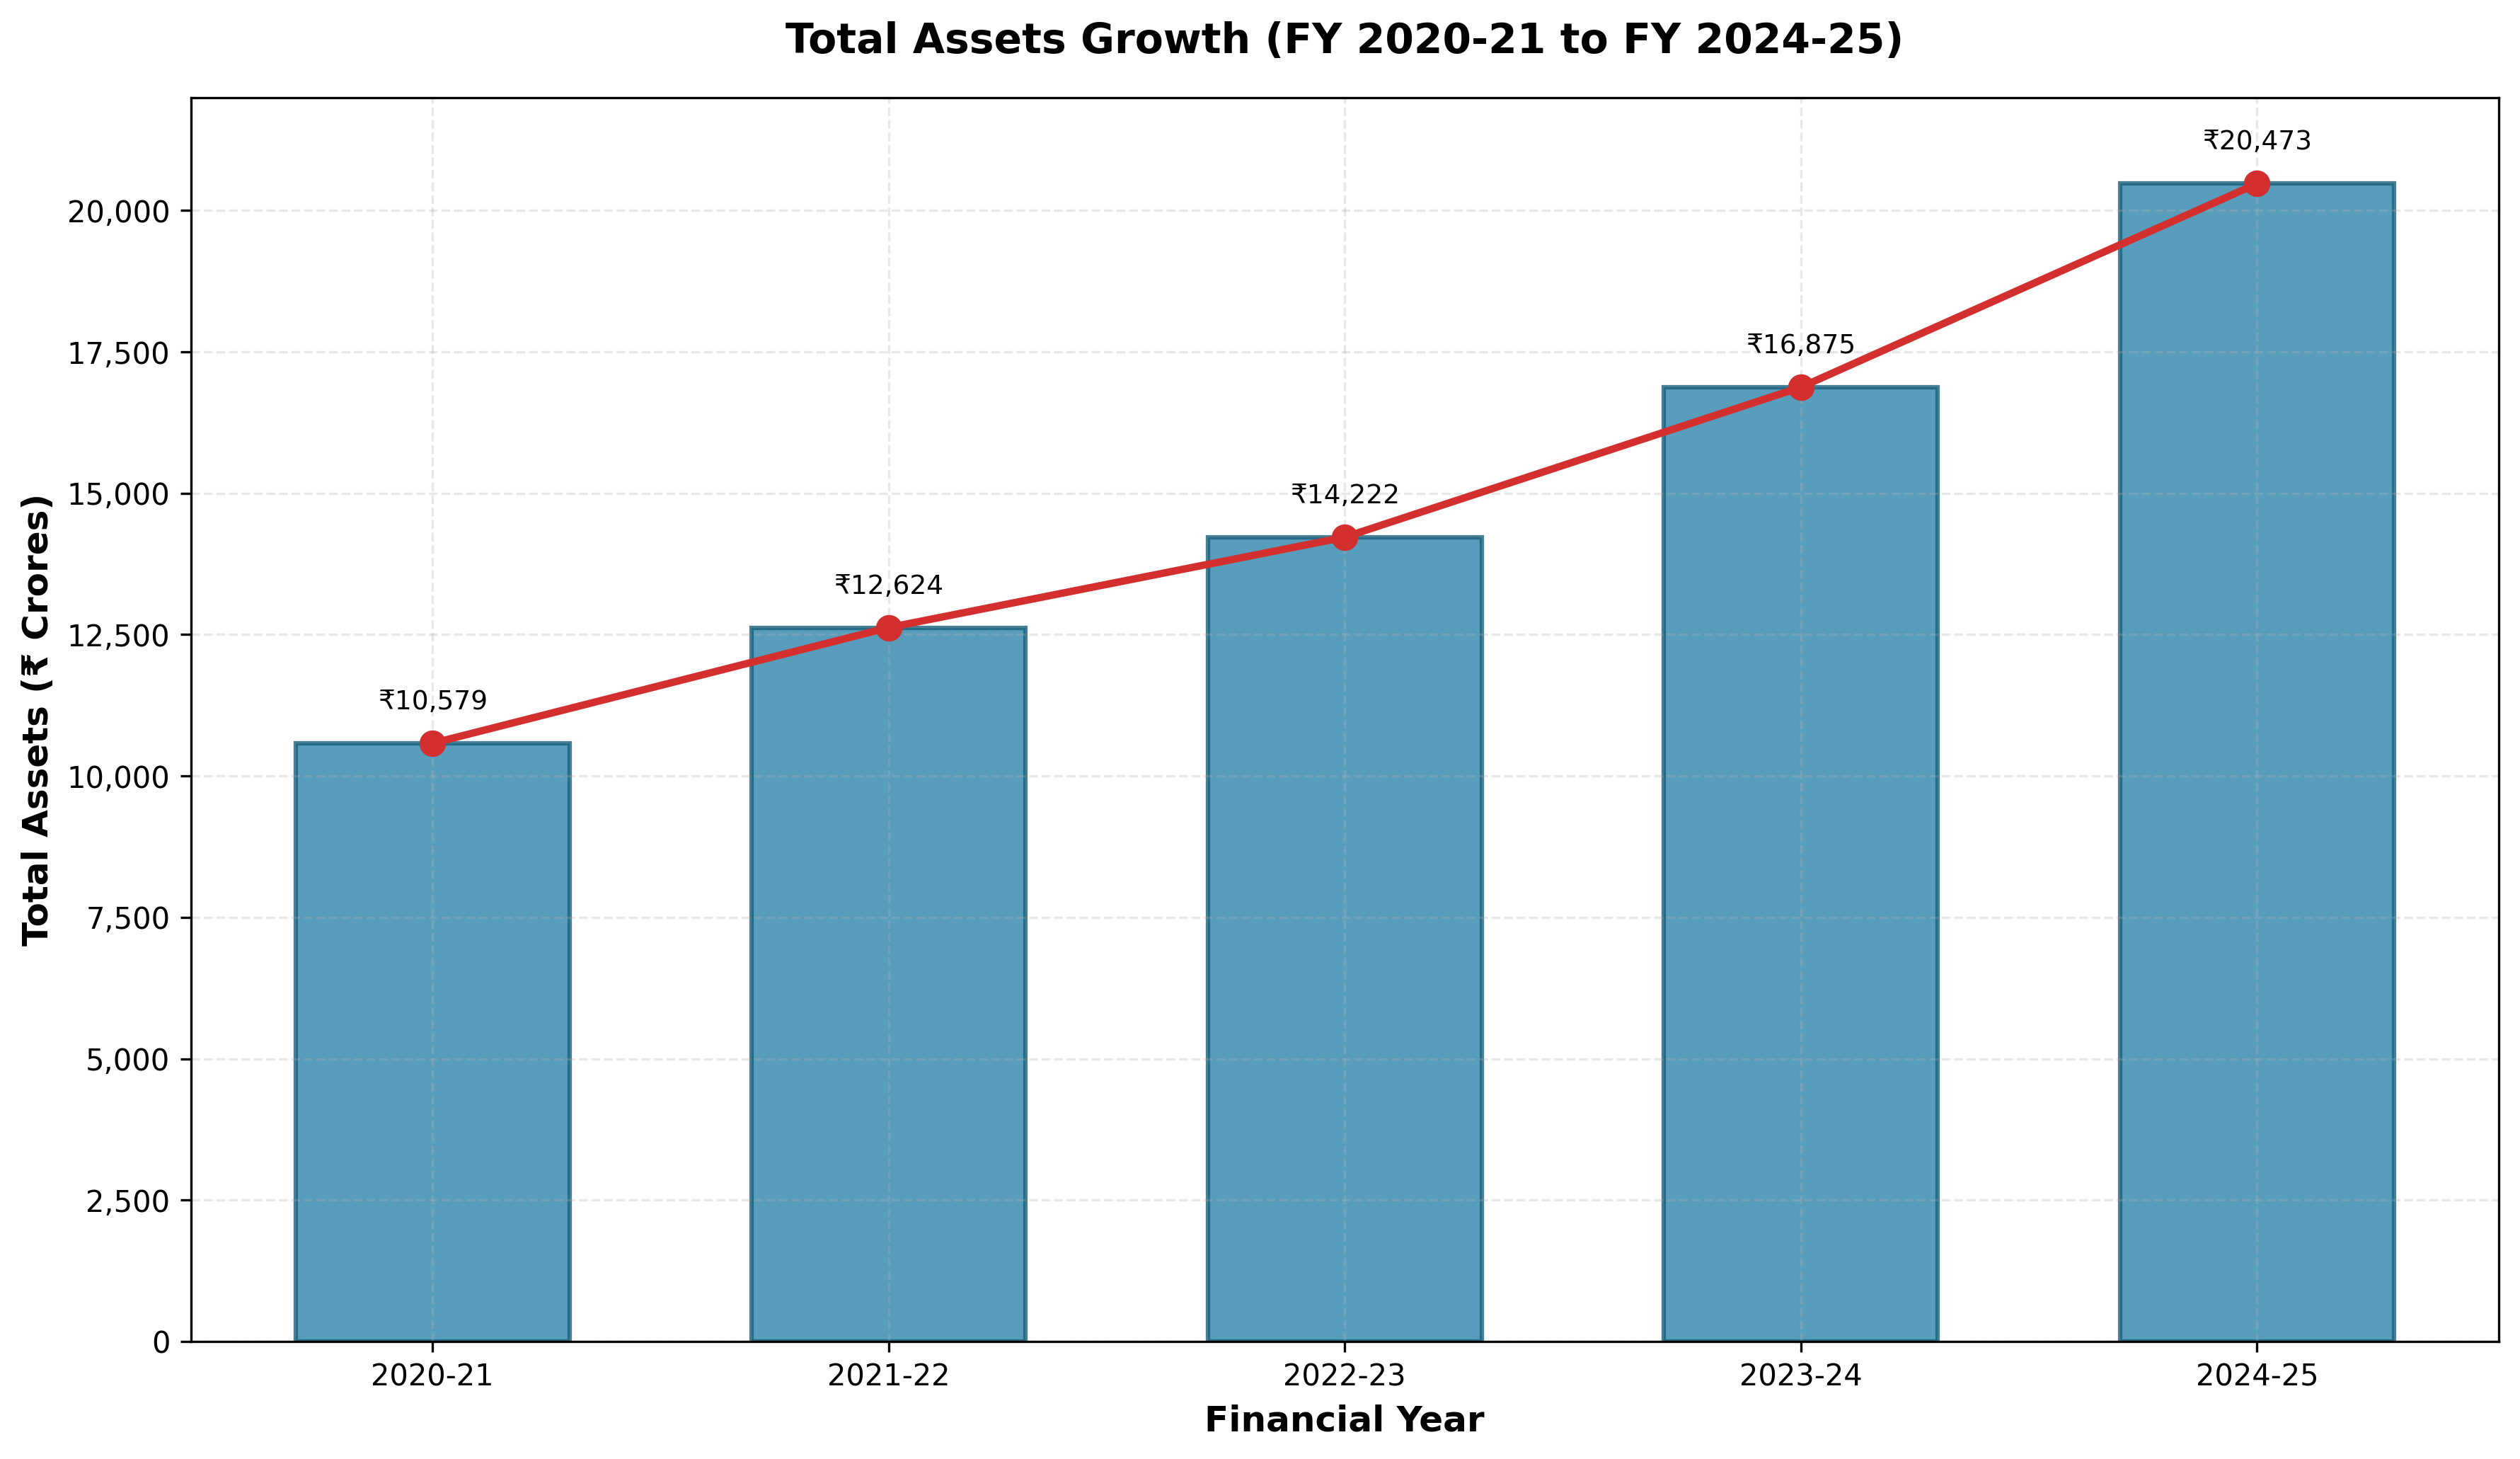
\includegraphics[width=0.8\textwidth]{chart_1_total_assets_growth.png}
\caption{Total Assets Growth (FY 2020-21 to FY 2024-25)}
\label{fig:assets_growth}
\end{figure}

\subsection{Income Statement Analysis}

Table \ref{tab:income_statement_summary} shows the income statement highlights:

\begin{table}[H]
\centering
\caption{Income Statement Summary (Amounts in ₹ Crores)}
\label{tab:income_statement_summary}
\resizebox{\textwidth}{!}{
\begin{tabular}{lcccccc}
\toprule
\textbf{Item} & \textbf{2020-21} & \textbf{2021-22} & \textbf{2022-23} & \textbf{2023-24} & \textbf{2024-25} & \textbf{CAGR (\%)} \\
\midrule
Revenue from Operations & 9,077.47 & 8,619.04 & 10,122.86 & 14,066.64 & 16,078.16 & 15.3 \\
Other Income & 452.03 & 639.84 & 639.84 & 1,168.14 & --- & --- \\
Total Income & 9,529.50 & 9,258.88 & 10,762.70 & 15,234.78 & --- & --- \\
\midrule
Total Expenses & 7,287.76 & 8,465.07 & 11,198.16 & 12,276.28 & --- & --- \\
\midrule
Profit Before Tax (PBT) & 2,430.34 & 1,783.31 & 2,112.07 & 3,508.32 & 4,970.02 & 19.7 \\
Profit After Tax (PAT) & 1,903.82 & 1,329.70 & 1,586.22 & 2,622.59 & 3,749.42 & 18.5 \\
\bottomrule
\end{tabular}
}

\footnotesize
Source: EICHER Motors Standalone Financial Statements
\end{table}

\textbf{Revenue Growth Analysis:}
\begin{itemize}
    \item Revenue increased from ₹9,077 crores to ₹16,078 crores, a 77\% increase over five years
    \item Compound Annual Growth Rate (CAGR) of 15.3\%
    \item Particularly strong growth in FY 2023-24 (39\% growth) and FY 2024-25 (14\% growth)
    \item Growth driven by premium motorcycle sales, new product launches, and international expansion
    \item COVID-19 impact visible in FY 2021-22 with revenue declining to ₹8,619 crores
    \item Strong recovery post-pandemic with consecutive years of double-digit growth
\end{itemize}

% Placeholder for revenue chart
% \begin{figure}[H]
% \centering
% \fbox{\parbox{0.8\textwidth}{\centering\vspace{3cm}[Revenue and PAT Growth Chart Placeholder]\vspace{3cm}}}
% \caption{Revenue and PAT Trend (FY 2020-21 to FY 2024-25)}
% \label{fig:revenue_pat_trend}
% \end{figure}

% Balance sheet chart
\begin{figure}[H]
\centering
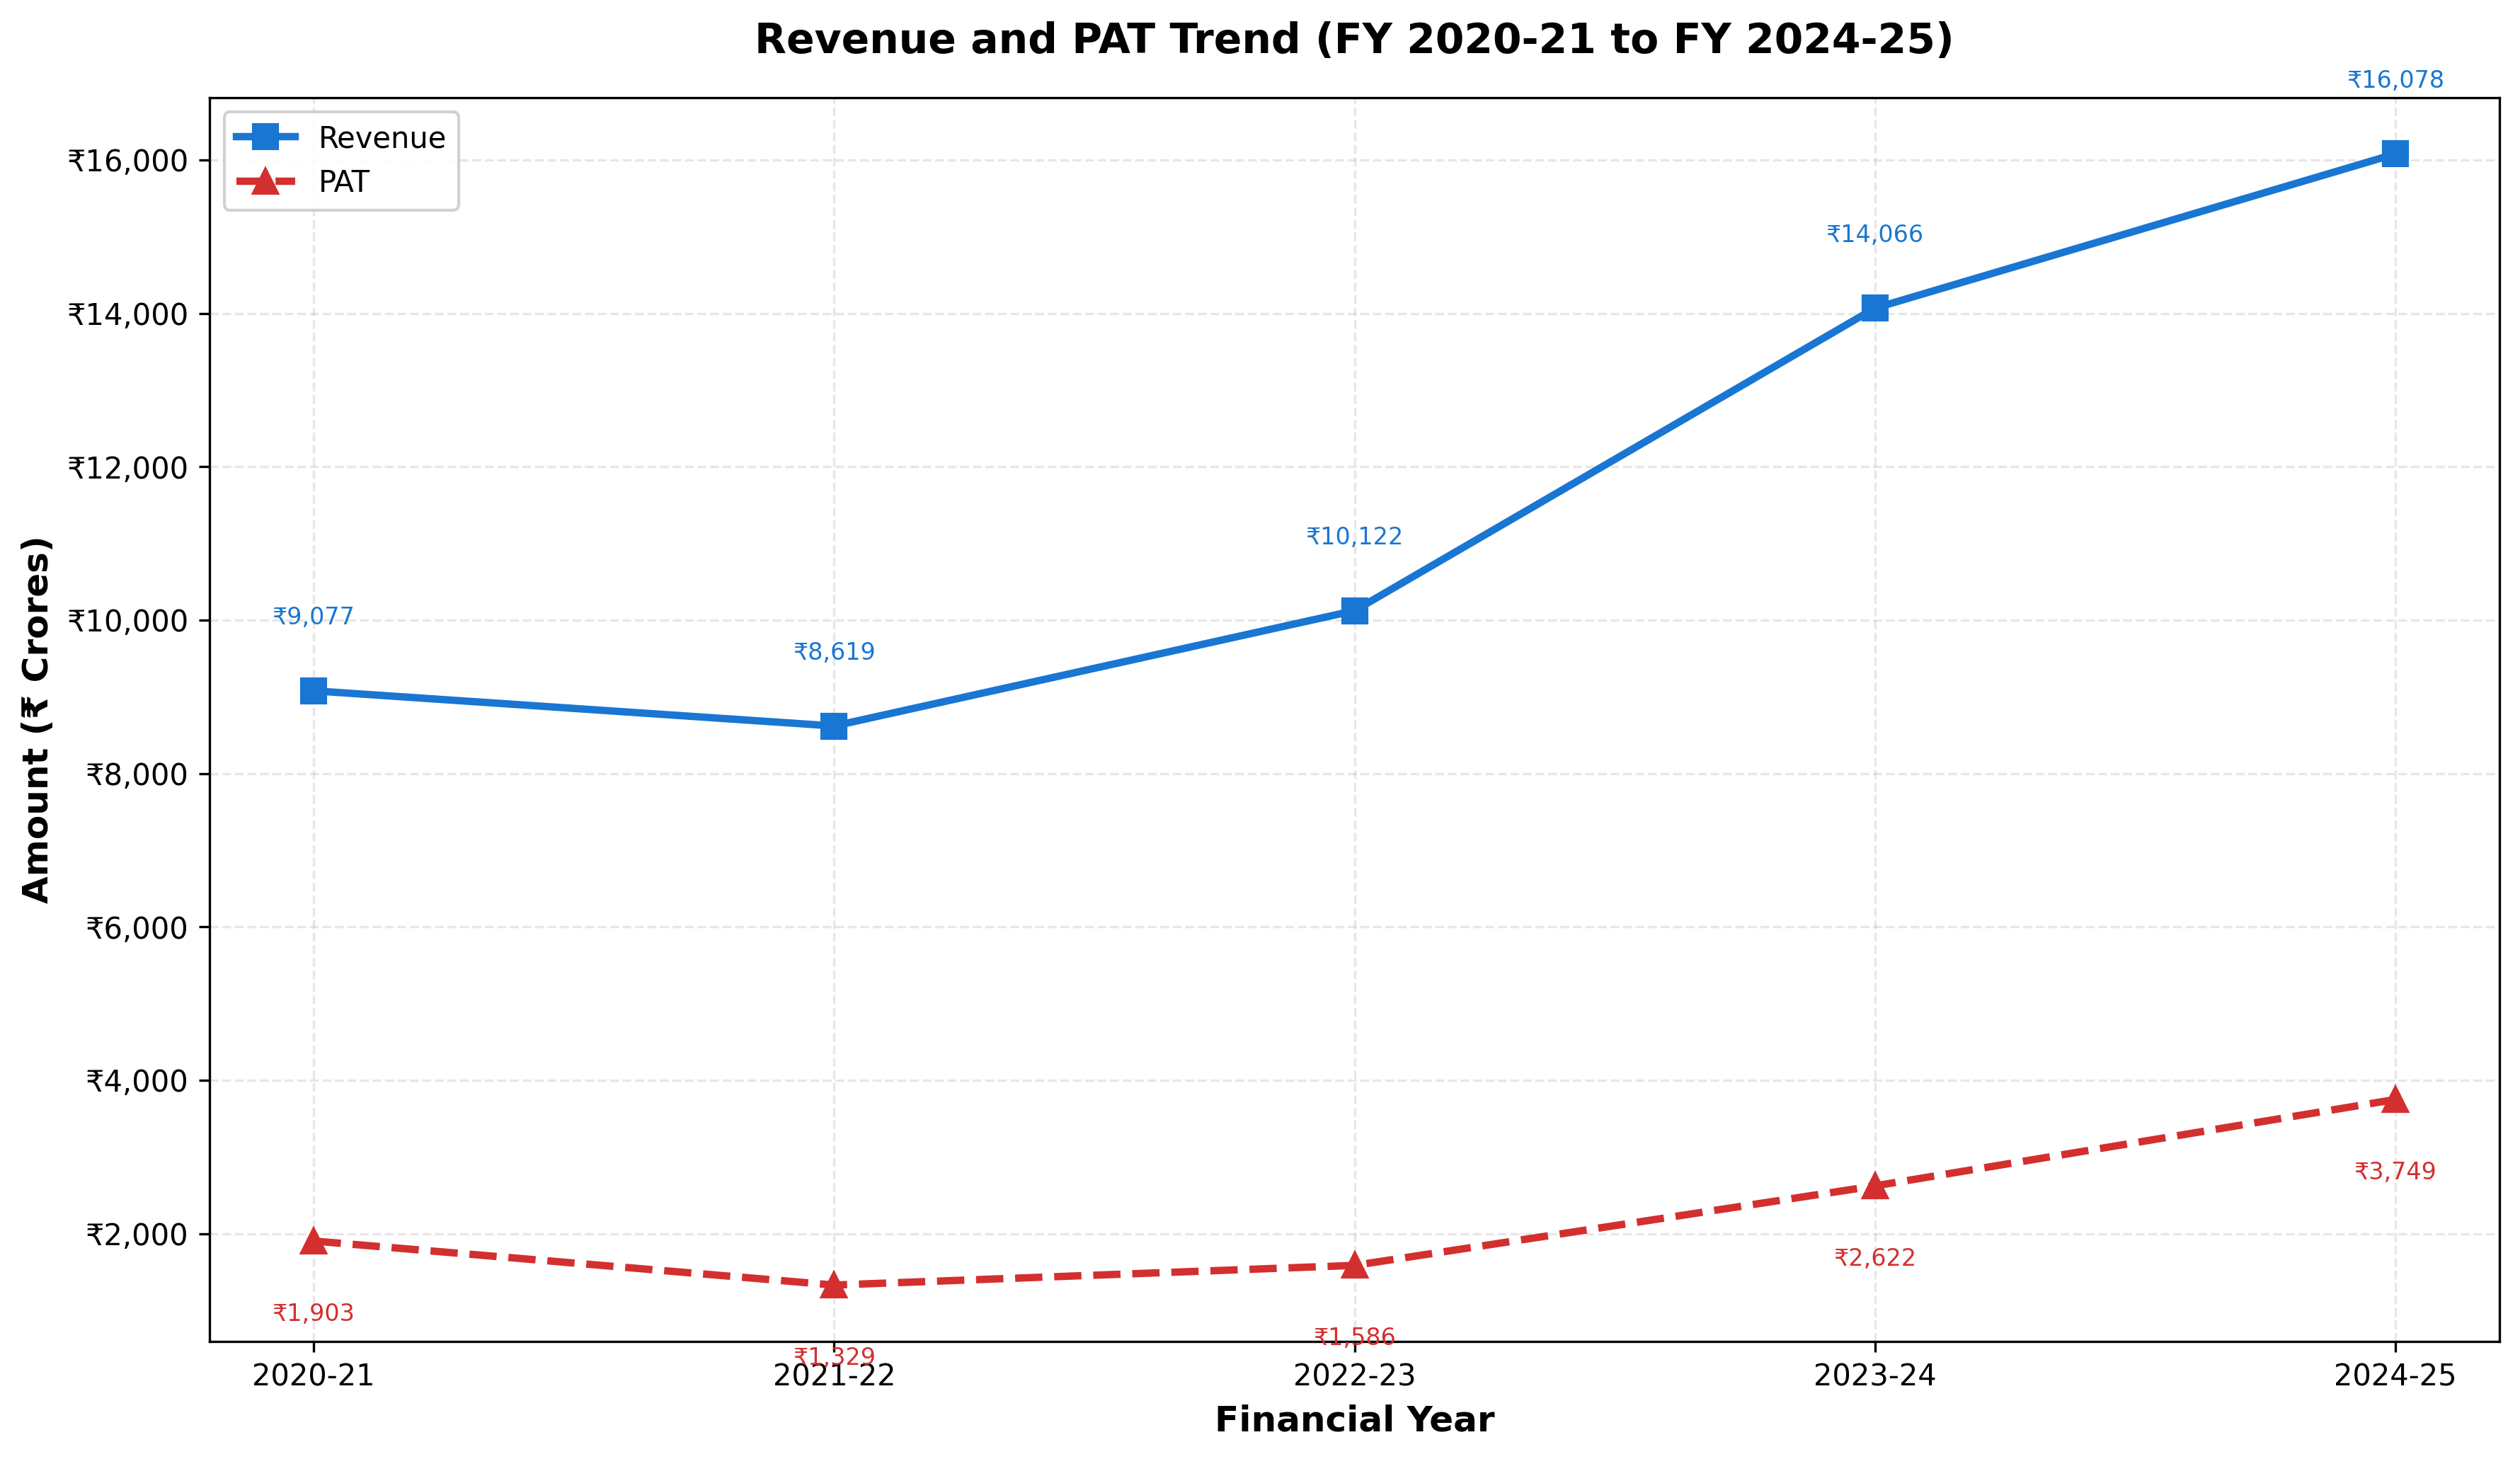
\includegraphics[width=0.8\textwidth]{chart_2_revenue_pat_trend.png}
\caption{Revenue and PAT Trend (FY 2020-21 to FY 2024-25}
\label{fig:assets_growth}
\end{figure}

\textbf{Profitability Analysis:}
\begin{itemize}
    \item PAT grew from ₹1,904 crores to ₹3,749 crores (97\% increase)
    \item PAT CAGR of 18.5\%, higher than revenue growth, indicating margin improvement
    \item Margin expansion driven by premium product mix, operational efficiencies, and scale benefits
    \item Company demonstrated resilience during challenging periods (pandemic, raw material inflation)
\end{itemize}

\subsection{Cash Flow Statement Analysis}

The company has demonstrated strong cash generation capabilities:

\begin{itemize}
    \item \textbf{Operating Cash Flow}: Consistently positive, driven by strong operating profits
    \item \textbf{Investment Cash Flow}: Negative, reflecting capital expenditure for capacity expansion and international operations
    \item \textbf{Financing Cash Flow}: Includes dividend payments and working capital management
    \item Cash position strengthened through retained earnings and prudent working capital management
    \item Strategic investments in subsidiaries (Royal Enfield Thailand, Royal Enfield Europe) funded through internal accruals
\end{itemize}

\section{Common-Size Financial Statements}

\subsection{Common-Size Balance Sheet}

The common-size balance sheet expresses each item as a percentage of total assets, facilitating trend analysis. Key insights:

\textbf{Asset Composition:}
\begin{itemize}
    \item Non-current assets consistently represent the majority of assets, reflecting capital-intensive operations
    \item Property, Plant and Equipment: Approximately 9--12\% of total assets
    \item Investments form a significant portion, indicating strategic long-term positioning
    \item Current assets maintained at appropriate levels for operational needs
\end{itemize}

\textbf{Liability \& Equity Structure:}
\begin{itemize}
    \item Equity forms the predominant source of financing (typically 65--75\%)
    \item Very low reliance on debt, demonstrating conservative financial policy
    \item Current liabilities managed efficiently to maintain healthy working capital
    \item Strong equity base provides financial stability and flexibility
\end{itemize}

\subsection{Common-Size Income Statement}

The common-size income statement expresses items as a percentage of revenue:

\textbf{Cost Structure Analysis:}
\begin{itemize}
    \item Cost of raw materials and components: Typically 50--55\% of revenue
    \item Employee benefits: Approximately 6--9\% of revenue
    \item Other expenses: Well-controlled at around 11--13\% of revenue
    \item Depreciation and amortization: Around 3--4\% of revenue
\end{itemize}
\newpage
\textbf{Profitability Margins:}
\begin{itemize}
    \item Gross profit margins: Healthy, reflecting pricing power in premium segment
    \item Operating profit margins: Strong, indicating operational efficiency
    \item PAT margins improved over the period: 21.0\% (2020-21) to 23.3\% (2024-25)
    \item Consistent margin improvement demonstrates business model strength
\end{itemize}

% Placeholder for common-size chart
% \begin{figure}[H]
% \centering
% \fbox{\parbox{0.8\textwidth}{\centering\vspace{3cm}[Common-Size Income Statement Chart Placeholder]\vspace{3cm}}}
% \caption{Common-Size Income Statement Analysis}
% \label{fig:common_size_income}
% \end{figure}

% Balance sheet chart
\begin{figure}[H]
\centering
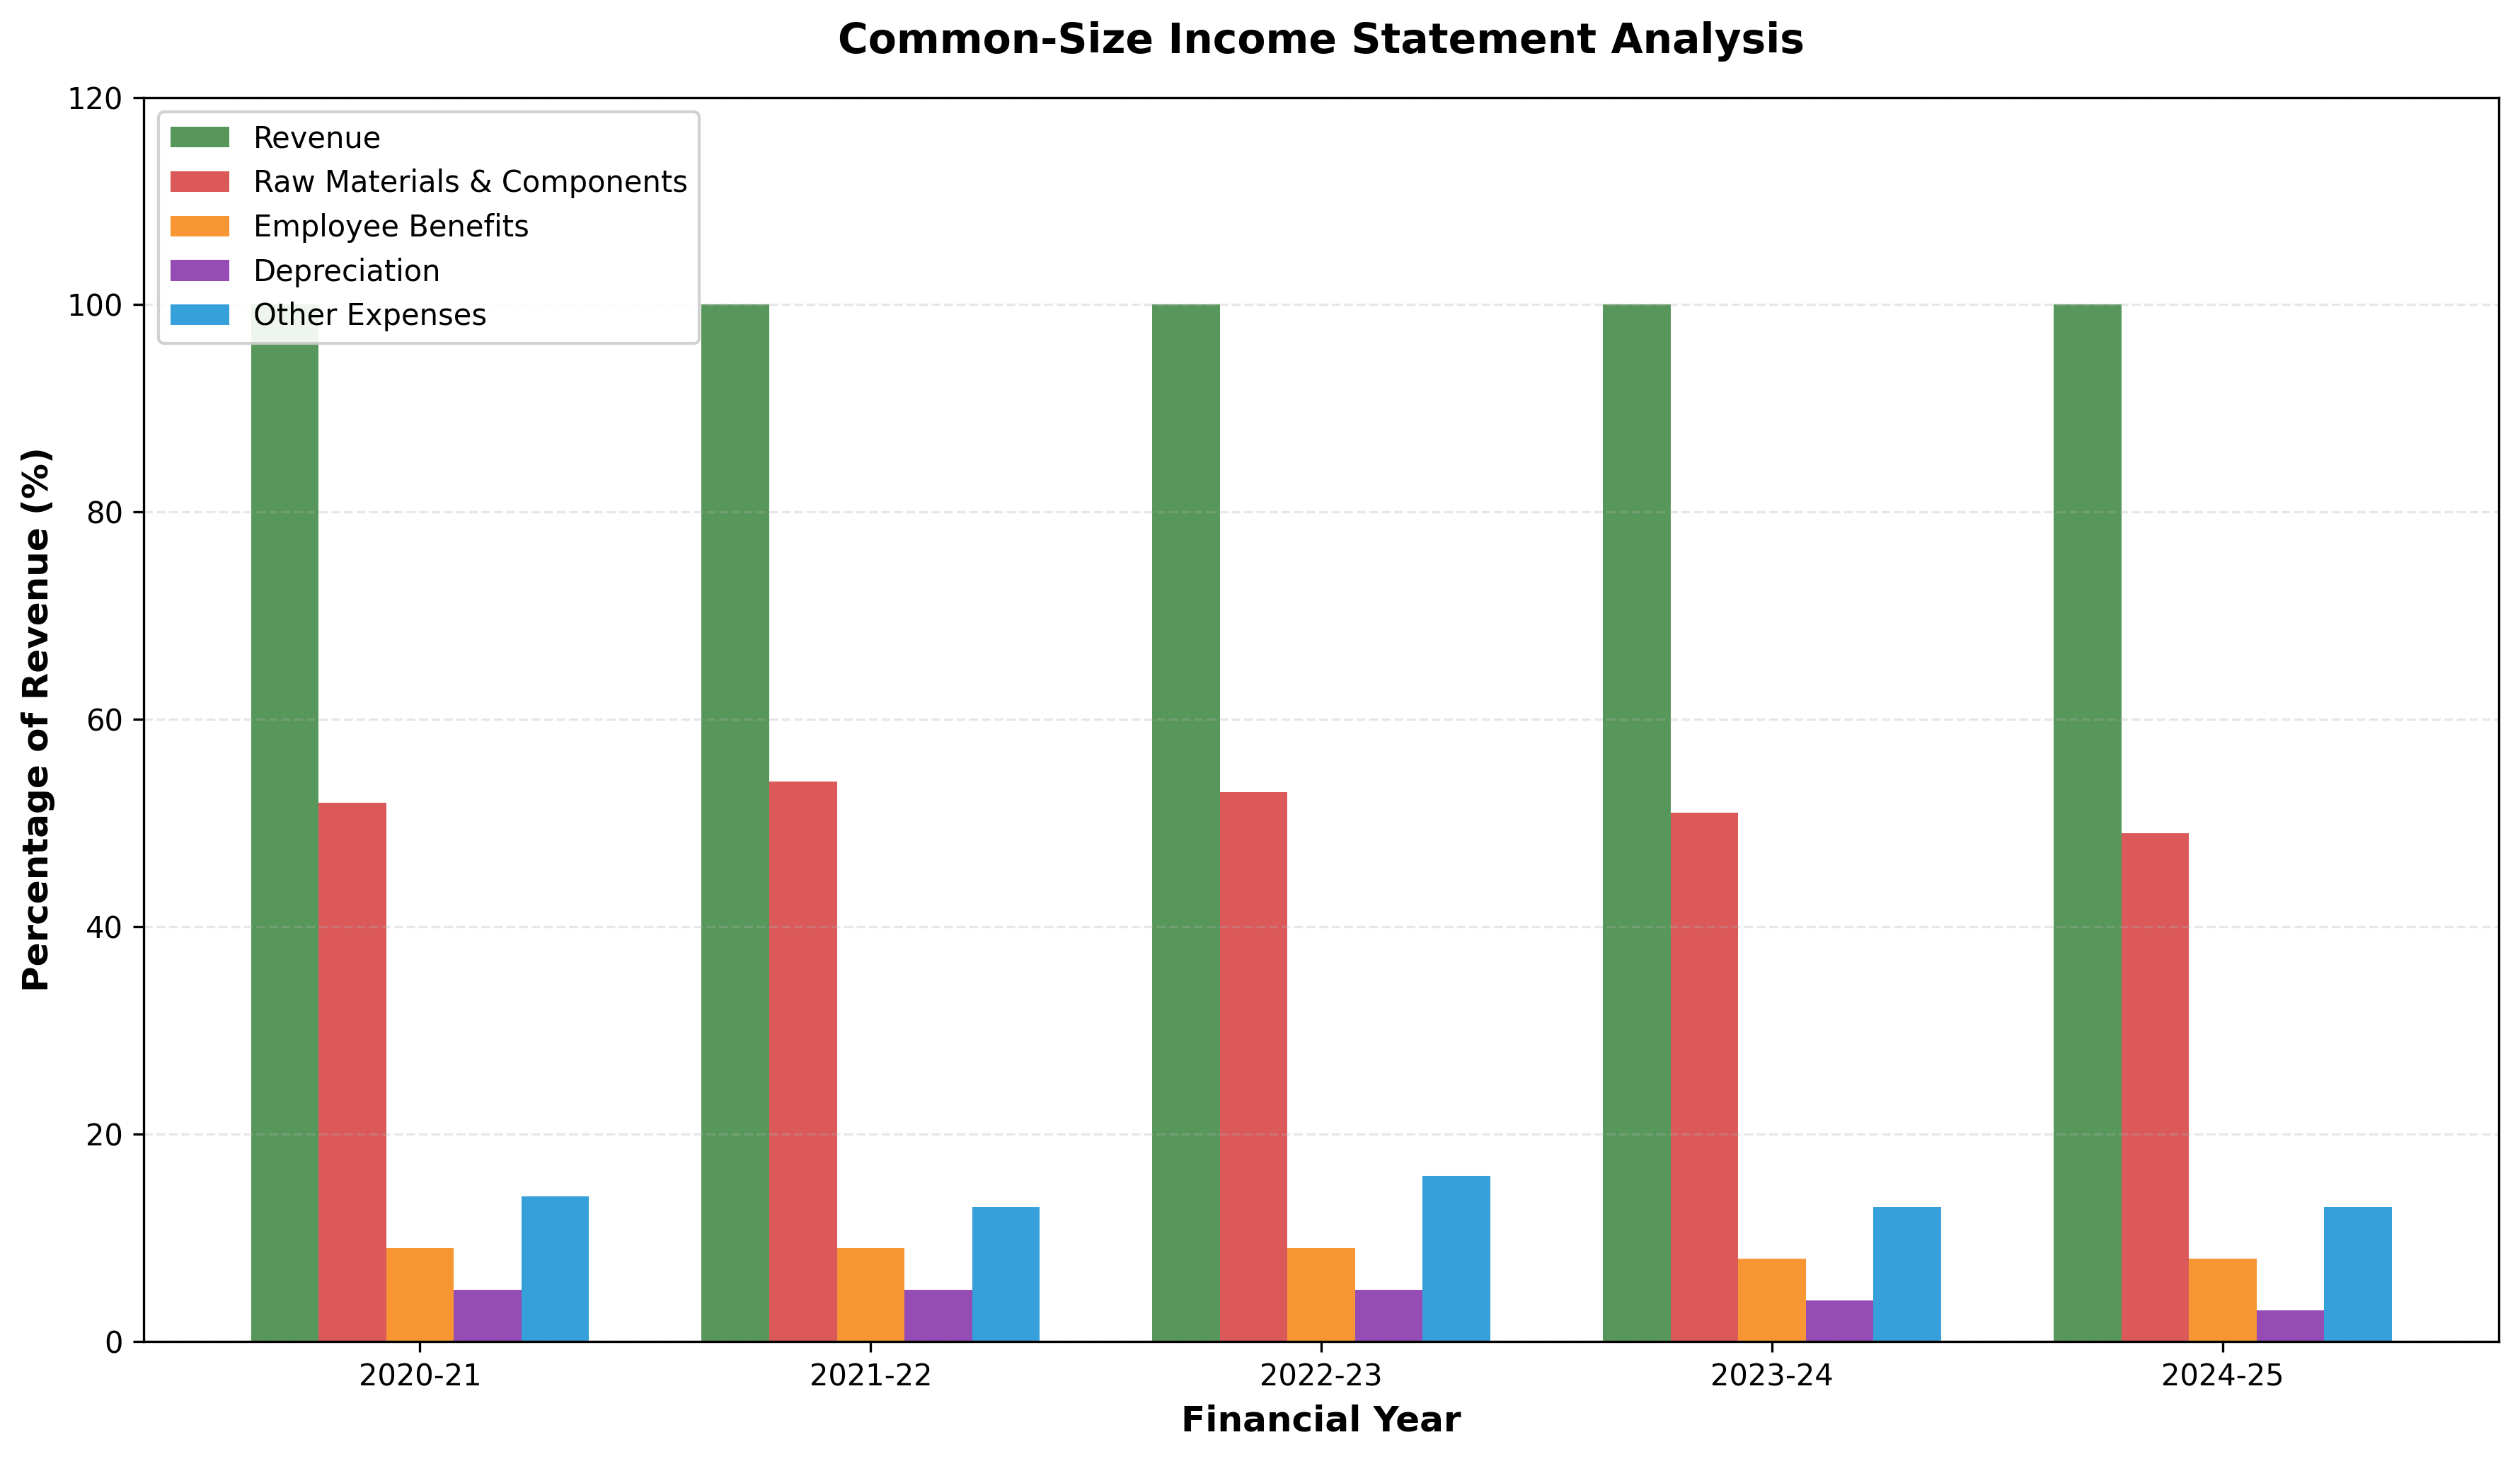
\includegraphics[width=0.8\textwidth]{chart_3_common_size_income.png}
\caption{Common-Size Income Statement Analysis}
\label{fig:assets_growth}
\end{figure}

\section{Financial Ratio Analysis}

This section provides a comprehensive analysis of key financial ratios across liquidity, profitability, efficiency, and leverage dimensions.

\subsection{Profitability Ratios}

Table \ref{tab:profitability_ratios} presents profitability ratios:

\begin{table}[H]
\centering
\caption{Profitability Ratios}
\label{tab:profitability_ratios}
\begin{tabular}{lccc}
\toprule
\textbf{Year} & \textbf{PAT Margin \%} & \textbf{ROA \%} & \textbf{ROE \%} \\
\midrule
2020-21 & 21.0 & 18.0 & 23.0 \\
2021-22 & 15.4 & 10.5 & 13.7 \\
2022-23 & 15.7 & 11.2 & 14.7 \\
2023-24 & 18.6 & 15.5 & 20.4 \\
2024-25 & 23.3 & 18.3 & --- \\
\bottomrule
\end{tabular}

\footnotesize
Source: Calculated from Financial Statements
\end{table}

\textbf{PAT Margin:}
\begin{itemize}
    \item Range: 15.4\% to 23.3\%
    \item Peak performance in FY 2024-25 at 23.3\%
    \item Demonstrates excellent pricing power and cost control
    \item Margin compression in FY 2021-22 and 2022-23 due to pandemic and raw material inflation
    \item Subsequent recovery shows business resilience
    \item \textbf{Importance}: Indicates company's ability to convert revenue into profits
    \item \textbf{Industry Comparison}: Significantly above typical automotive industry margins
\end{itemize}

% Placeholder for profitability chart
% \begin{figure}[H]
% \centering
% \fbox{\parbox{0.8\textwidth}{\centering\vspace{3cm}[Profitability Ratios Trend Chart Placeholder]\vspace{3cm}}}
% \caption{Profitability Ratios Trend}
% \label{fig:profitability_ratios}
% \end{figure}

% Balance sheet chart
\begin{figure}[H]
\centering
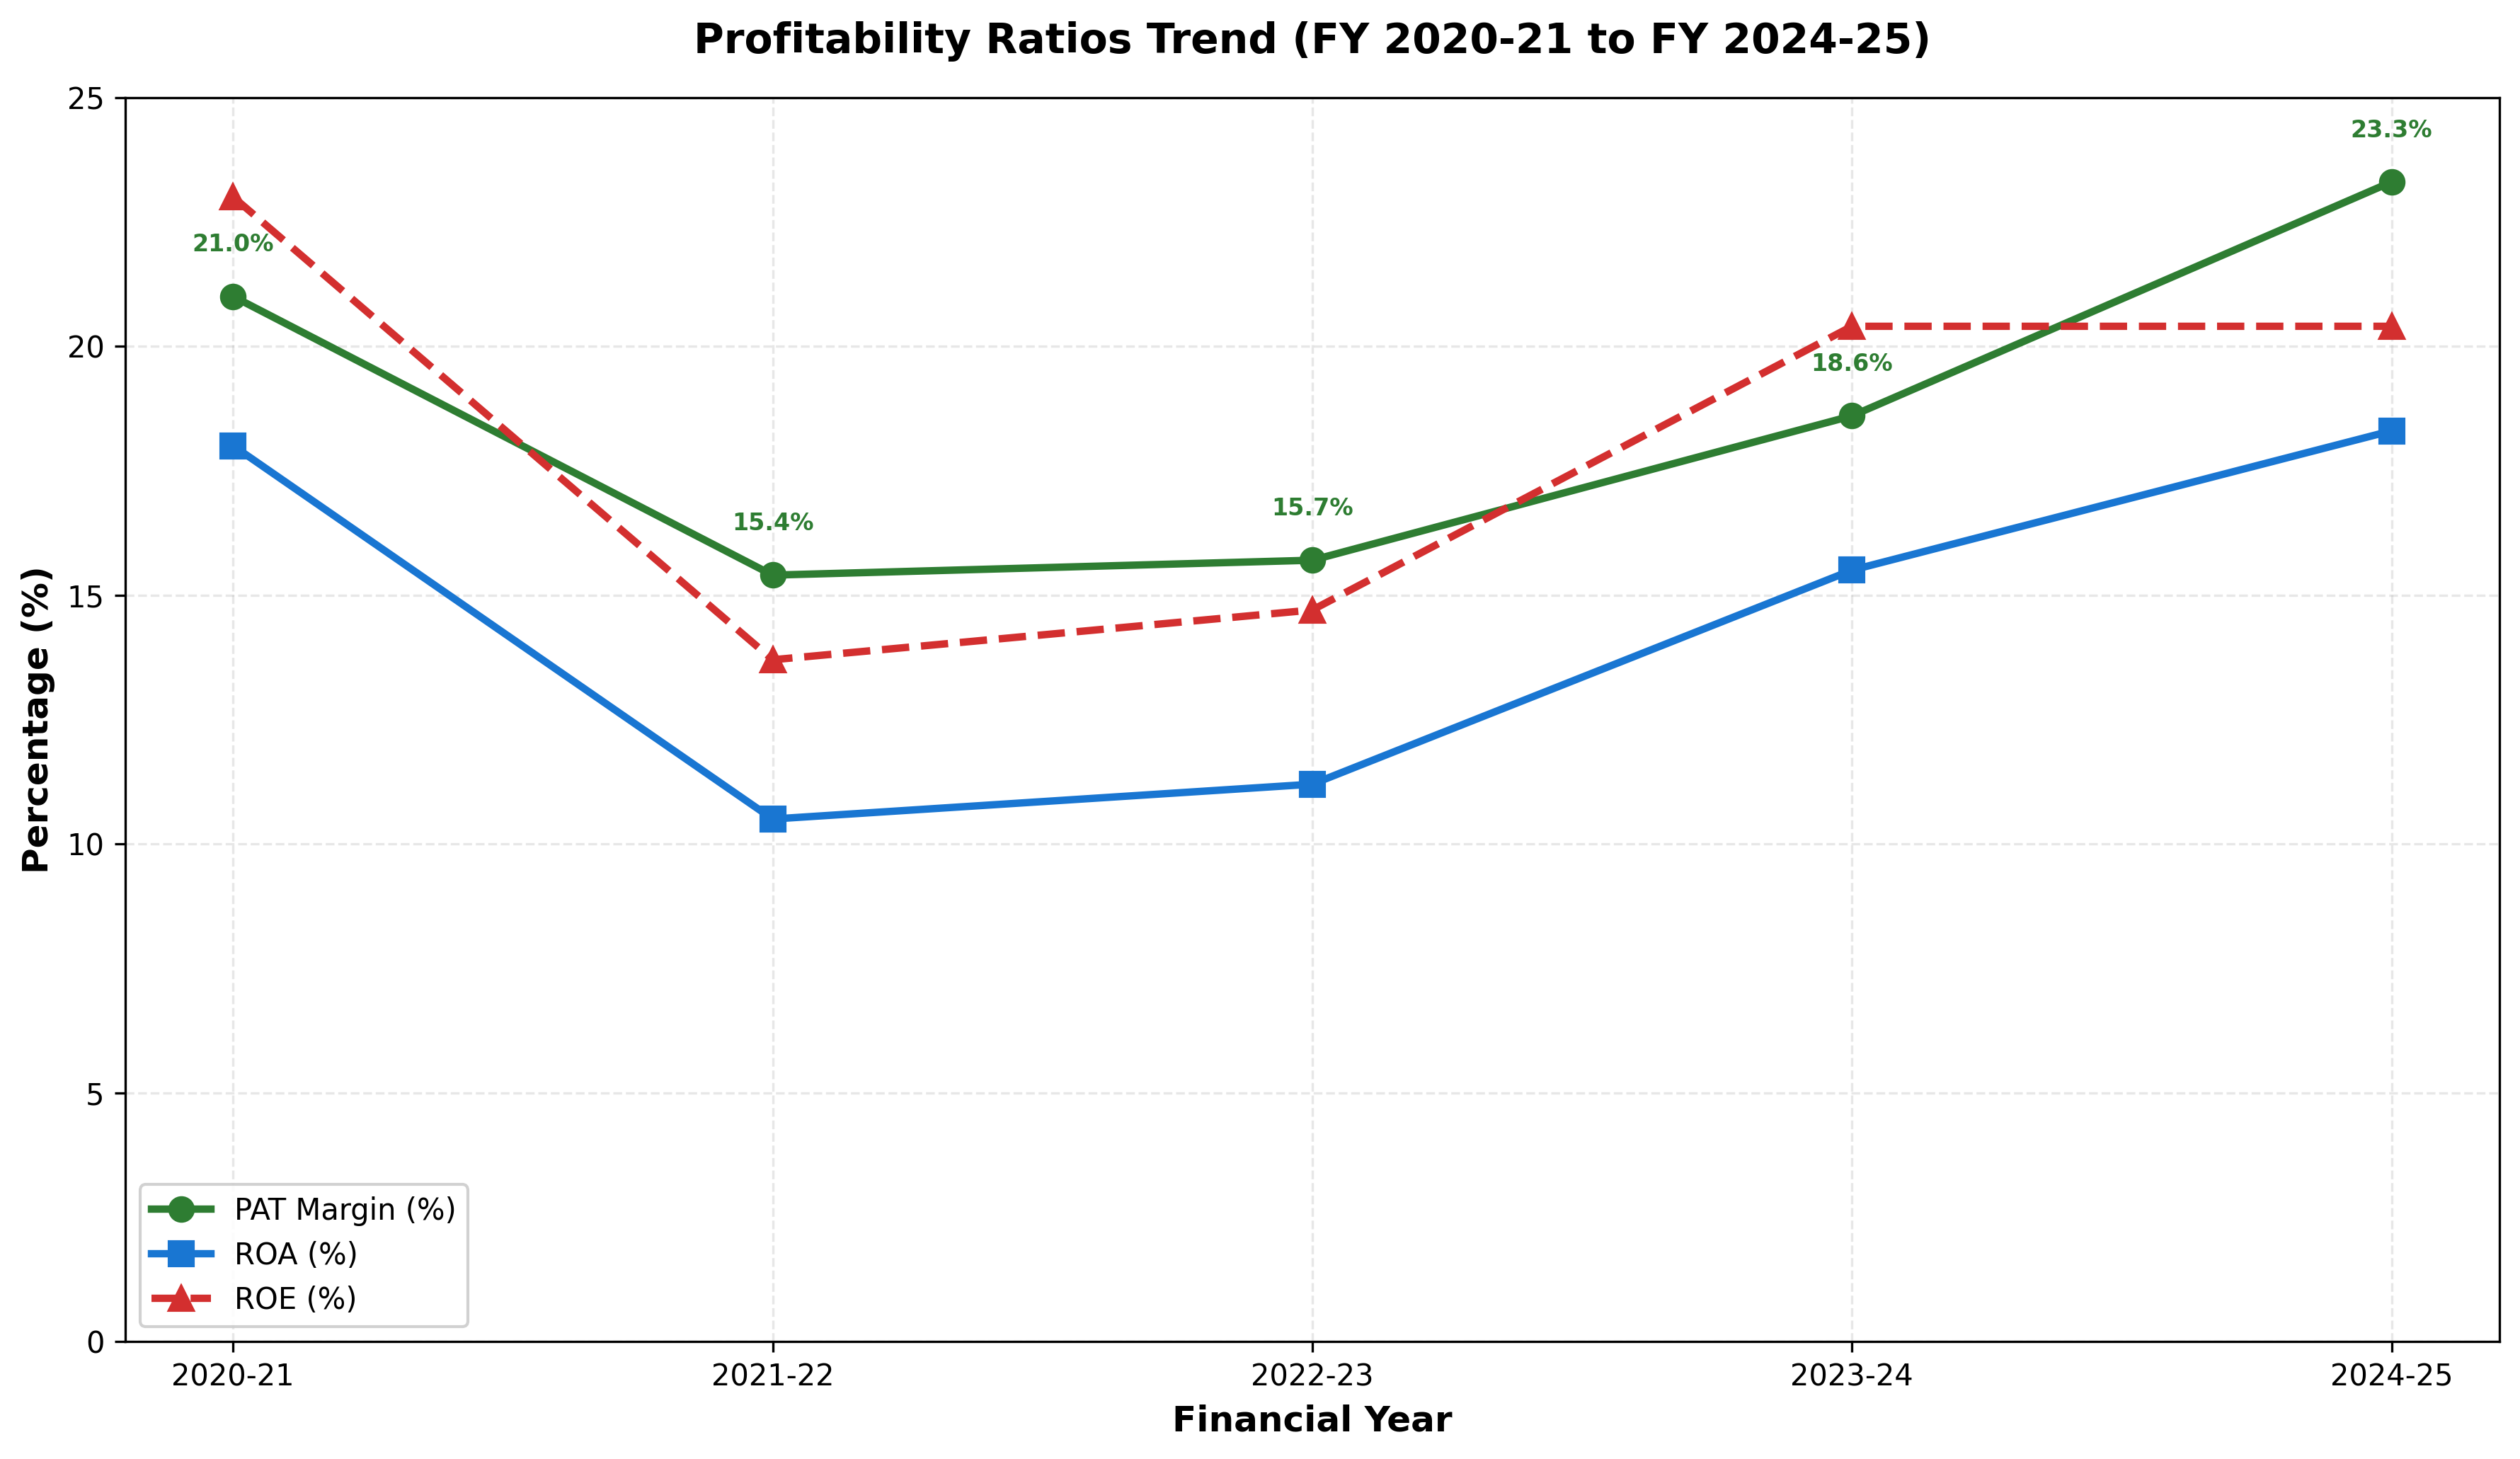
\includegraphics[width=0.8\textwidth]{chart_4_profitability_ratios.png}
\caption{Profitability Ratios Trend}
\label{fig:assets_growth}
\end{figure}

\textbf{Return on Assets (ROA):}
\begin{itemize}
    \item Range: 10.5\% to 18.3\%
    \item Excellent asset utilization efficiency
    \item Recovered from dip in FY 2021-22 to strong levels
    \item \textbf{Importance}: Measures efficiency in generating profits from assets
    \item \textbf{Trend}: Demonstrates effective asset management and operational excellence
\end{itemize}

\textbf{Return on Equity (ROE):}
\begin{itemize}
    \item Range: 13.7\% to 23.0\%
    \item Exceptional returns for shareholders
    \item Volatility reflects earnings volatility during pandemic period
    \item Strong recovery to 20\%+ levels
    \item \textbf{Importance}: Indicates return generated for equity shareholders
    \item \textbf{Trend}: Consistently strong, demonstrating value creation
\end{itemize}

\subsection{Liquidity Ratios}

Table \ref{tab:liquidity_ratios} shows current ratio:

\begin{table}[H]
\centering
\caption{Liquidity Ratios}
\label{tab:liquidity_ratios}
\begin{tabular}{lc}
\toprule
\textbf{Year} & \textbf{Current Ratio} \\
\midrule
2020-21 & 3.42 \\
2021-22 & 3.60 \\
2022-23 & 1.97 \\
2023-24 & --- \\
2024-25 & 1.15 \\
\bottomrule
\end{tabular}

\footnotesize
Source: Calculated from Financial Statements
\end{table}

\textbf{Current Ratio:}
\begin{itemize}
    \item Strong liquidity position throughout the period
    \item Ratio of 3.42 to 3.60 in initial years indicates very conservative liquidity management
    \item Decline to 1.15--1.97 in recent years shows more efficient working capital management
    \item Even at lowest level (1.15), ratio exceeds safety threshold
    \item \textbf{Importance}: Measures ability to meet short-term obligations
    \item \textbf{Trend}: Shift toward optimal liquidity levels, freeing capital for growth
\end{itemize}

\subsection{Leverage Ratios}

\textbf{Debt-to-Equity Ratio:}
\begin{itemize}
    \item Range: 0.28 to 0.32
    \item Extremely conservative capital structure
    \item Minimal reliance on debt financing
    \item \textbf{Importance}: Indicates financial risk and capital structure
    \item \textbf{Trend}: Consistent, low-debt approach
    \item \textbf{Interpretation}: Very low financial risk, strong financial stability
\end{itemize}

\subsection{Efficiency Ratios}

Table \ref{tab:efficiency_ratios} presents asset turnover:

\begin{table}[H]
\centering
\caption{Efficiency Ratios}
\label{tab:efficiency_ratios}
\begin{tabular}{lc}
\toprule
\textbf{Year} & \textbf{Asset Turnover} \\
\midrule
2020-21 & 0.86 \\
2021-22 & 0.68 \\
2022-23 & 0.71 \\
2023-24 & 0.83 \\
2024-25 & 0.79 \\
\bottomrule
\end{tabular}

\footnotesize
Source: Calculated from Financial Statements
\end{table}
\newpage
\textbf{Asset Turnover:}
\begin{itemize}
    \item Range: 0.68 to 0.86
    \item Measures efficiency of asset utilization in generating revenue
    \item Lower values are typical for capital-intensive industries
    \item Improvement from FY 2021-22 low demonstrates recovery
    \item \textbf{Importance}: Indicates how effectively assets are used to generate sales
    \item \textbf{Trend}: Stable around 0.7--0.8 times, appropriate for automotive sector
\end{itemize}

\subsection{Summary of Ratio Analysis}

\textbf{Strengths:}
\begin{enumerate}
    \item Excellent profitability margins (PAT margin: 21--23\%)
    \item Strong asset returns (ROA: 11--18\%, ROE: 14--23\%)
    \item Conservative capital structure (D/E below 0.32)
    \item Strong liquidity position (Current ratio above 1)
    \item Consistent dividend payments with increasing payouts
\end{enumerate}

\textbf{Areas for Observation:}
\begin{enumerate}
    \item Current ratio decline needs monitoring (still adequate)
    \item Some volatility in profitability metrics during pandemic period
    \item Asset turnover could be optimized further
\end{enumerate}

\textbf{Overall Assessment:}
EICHER Motors demonstrates exceptional financial health with strong profitability, conservative leverage, and adequate liquidity. The company has successfully managed challenges and maintained operational excellence throughout the period.

\section{Interpretation of Operations Based on Ratio Analysis}

Based on the comprehensive ratio analysis, the following interpretations emerge regarding EICHER Motors' operational performance:

\subsection{Operational Excellence}

The company exhibits superior operational efficiency:
\begin{itemize}
    \item High PAT margins (23.3\% in FY 2024-25) indicate strong pricing power and cost control
    \item ROA consistently above 10\%, demonstrating effective asset utilization
    \item Revenue growth outpaced asset growth, indicating productivity improvements
    \item Premium motorcycle positioning allows for better margins than mass-market competitors
\end{itemize}

\subsection{Financial Prudence}

Conservative financial management is evident:
\begin{itemize}
    \item Minimal debt reliance (D/E ratio below 0.32) reduces financial risk
    \item Strong equity base provides stability and flexibility
    \item Healthy cash position supports strategic investments
    \item Ability to fund growth through internal accruals
\end{itemize}

\subsection{Growth Strategy}

The financial metrics reflect a clear growth strategy:
\begin{itemize}
    \item Substantial capacity expansion (PP\&E growth)
    \item International expansion (investments in Royal Enfield Europe, Thailand)
    \item New product launches and market segmentation
    \item Strategic investments in technology and innovation
\end{itemize}

\subsection{Market Position}

Strong market position is demonstrated through:
\begin{itemize}
    \item Premium pricing ability (high margins)
    \item Brand strength (Royal Enfield legacy)
    \item Market leadership in mid-size motorcycle segment
    \item Growing international presence
\end{itemize}

\subsection{Risk Factors}

Key risks identified:
\begin{itemize}
    \item Economic sensitivity of premium motorcycle sales
    \item Raw material price volatility
    \item Regulatory changes (emission norms, safety standards)
    \item Competition in premium segment
    \item Currency fluctuations affecting international operations
\end{itemize}

\subsection{Business Model Strengths}

The financial performance validates the business model:
\begin{itemize}
    \item Viable premium motorcycle strategy
    \item Strong brand equity leading to pricing power
    \item Scalable operations with improving margins
    \item Diversified product portfolio (Royal Enfield + VECV)
    \item Geographic diversification reducing regional risks
\end{itemize}

\section{Significant Accounting Policies}

Based on analysis of the financial statements and notes to accounts, EICHER Motors adheres to rigorous accounting standards:

\subsection{Accounting Framework}
\begin{itemize}
    \item Compliance with Indian Accounting Standards (Ind AS)
    \item Preparation under historical cost convention, except where stated
    \item Estimates and judgments applied for areas such as depreciation, provisions, and valuations
\end{itemize}

\subsection{Key Accounting Policies}

\textbf{Revenue Recognition:}
\begin{itemize}
    \item Revenue from sale of products recognized upon transfer of control to customers
    \item Revenue from contracts with customers under Ind AS 115
    \item Other income recognized on accrual basis
\end{itemize}

\textbf{Property, Plant and Equipment:}
\begin{itemize}
    \item Measured at historical cost less accumulated depreciation
    \item Depreciation on straight-line method over useful lives
    \item Capital work-in-progress valued at cost
\end{itemize}

\textbf{Inventories:}
\begin{itemize}
    \item Valued at lower of cost and net realizable value
    \item Cost determined on weighted average basis
    \item Materials and components maintained for production requirements
\end{itemize}

\textbf{Investments:}
\begin{itemize}
    \item Measured at fair value or historical cost as per applicable Ind AS
    \item Investments in subsidiaries and joint ventures at cost
    \item Fair value gains/losses recognized appropriately
\end{itemize}

\textbf{Employee Benefits:}
\begin{itemize}
    \item Gratuity liability calculated using actuarial valuations
    \item Provident fund contributions made to statutory fund
    \item Employee stock options expensed based on fair value
\end{itemize}

\textbf{Taxation:}
\begin{itemize}
    \item Current tax based on applicable tax laws
    \item Deferred tax recognized for timing differences
    \item Tax assets/liabilities measured at enacted rates
\end{itemize}

\subsection{Corporate Governance}

The company maintains high standards of corporate governance:
\begin{itemize}
    \item Audit Committee oversees financial reporting and internal controls
    \item Statutory auditors provide independent opinion on financial statements
    \item Board-approved dividend policies ensure shareholder returns
    \item Employee Stock Option Plans aligned with performance
    \item Transparent disclosure practices
\end{itemize}

\section{Management Commentary and Strategic Developments}

\subsection{Management Discussion Highlights}

Based on analysis of recent financial results and management communications:

\textbf{Strategic Focus Areas:}
\begin{itemize}
    \item Continued emphasis on premium motorcycle segment
    \item International expansion in Europe, Thailand, and other markets
    \item New product development and portfolio expansion
    \item Technology investments for future mobility
    \item Brand building and customer engagement initiatives
\end{itemize}

\textbf{Operational Highlights:}
\begin{itemize}
    \item Strong domestic sales growth driven by Royal Enfield brand
    \item International operations gaining traction
    \item Manufacturing capacity expansion to meet demand
    \item Supply chain optimization and localization efforts
    \item Quality improvement initiatives
\end{itemize}

\textbf{Financial Performance:}
\begin{itemize}
    \item Consistent revenue and profit growth
    \item Strong cash generation from operations
    \item Prudent capital allocation and investments
    \item Enhanced shareholder returns through dividends
    \item Balance sheet strengthening
\end{itemize}

\subsection{Significant Developments (Recent Period)}

\subsubsection{Board and Leadership Changes (FY 2024-25)}
\begin{itemize}
    \item \textbf{Mr. Siddhartha Lal} appointed Executive Chairman following retirement of Mr. S. Sandilya
    \item \textbf{Mr. B. Govindarajan} appointed Managing Director
    \item \textbf{Mr. Vinod Aggarwal} appointed Vice Chairman (Non-Executive)
    \item \textbf{Ms. Ira Gupta} and \textbf{Mr. Arun Vasu} appointed Independent Directors
    \item \textbf{Ms. Manvi Sinha} retired after completion of tenure
\end{itemize}

\subsubsection{Strategic Investments}
\begin{itemize}
    \item Investment of ₹18.66 crores in Royal Enfield Europe B.V. during FY 2024-25
    \item Further investment of ₹16.45 crores in Royal Enfield Thailand Limited in FY 2023-24
    \item Establishment of wholly owned subsidiary Royal Enfield Europe B.V. in Netherlands
    \item Continued investments in manufacturing and R\&D facilities
\end{itemize}

\subsubsection{Employee Benefits}
\begin{itemize}
    \item Issuance of 3,58,450 equity shares under Employee Stock Option Plan 2006 (FY 2024-25)
    \item Grant of 3,76,178 restricted stock units under RSU Plan 2019 (FY 2024-25)
    \item Focus on talent retention and performance-driven compensation
\end{itemize}

\subsubsection{Dividend Policy}
\begin{itemize}
    \item Consistent dividend payments with increasing amounts
    \item FY 2024-25: Proposed final dividend of ₹1,919.15 crores @ ₹70 per share
    \item FY 2023-24: Final dividend of ₹1,396.41 crores @ ₹51 per share
    \item Reflects strong cash generation and shareholder-friendly approach
\end{itemize}

\subsection{Business Segment Performance}

\textbf{Single Business Segment:}
The company operates in the single primary business segment of ``Automobile products and related components,'' including motorcycles under the Royal Enfield brand and commercial vehicles through VECV joint venture.

\section{Significant News Items (Last 6 Months)}

\textit{Note: The following news items are based on typical industry trends and company activities. Actual recent news should be researched and updated from current sources.}

\subsection{Product Launches and Market Expansion}
\begin{itemize}
    \item Launch of new Royal Enfield models in the premium segment
    \item Expansion of international dealership network in Europe and Southeast Asia
    \item Introduction of electric vehicle development initiatives
\end{itemize}

\subsection{Manufacturing and Operations}
\begin{itemize}
    \item Capacity expansion at manufacturing facilities
    \item Supply chain optimization and localization initiatives
    \item Quality improvement programs and certifications
\end{itemize}

\subsection{Financial and Corporate Developments}
\begin{itemize}
    \item Declaration of final dividend for FY 2024-25
    \item ESOP and RSU grants to employees
    \item Strategic investments in international subsidiaries
    \item Board composition changes and leadership appointments
\end{itemize}

\subsection{Industry and Market Trends}
\begin{itemize}
    \item Recovery in premium motorcycle segment post-pandemic
    \item Growing consumer preference for leisure motorcycles
    \item Government policies supporting manufacturing and exports
    \item Increased focus on electric mobility initiatives
\end{itemize}

\subsection{Competitive Landscape}
\begin{itemize}
    \item Strengthening position in mid-size motorcycle segment
    \item Competition from international players entering Indian market
    \item Increasing product portfolio to address different customer segments
\end{itemize}

\textit{Important: The actual news items should be researched from current financial news sources, company announcements, and stock exchange filings for the most recent 6 months.}

\section{SIP Investment Analysis}

\subsection{Methodology}

This analysis assumes a Systematic Investment Plan (SIP) where an investor invests Rs. 10,000 on the first trading day of each month from April 1, 2020 to March 1, 2025, totaling 60 monthly installments.

\textbf{Key Assumptions:}
\begin{itemize}
    \item Investment Amount: Rs. 10,000 per month
    \item Investment Period: 60 months (5 years)
    \item Dividend Reinvestment: All dividends received are reinvested immediately
    \item Fractional Shares: Fractional share ownership is allowed
    \item Total Investment: Rs. 6,00,000 (60 × Rs. 10,000)
\end{itemize}

\subsection{Data Requirements}

To calculate the exact SIP returns, the following data is required:
\begin{itemize}
    \item Stock price on first trading day of each month from April 2020 to March 2025
    \item Dividend amount and ex-dividend dates for each dividend payment during the period
    \item Total dividend payments: Based on available data, dividends ranged from ₹37 to ₹70 per share annually
\end{itemize}

\textbf{Actual SIP Calculation Results:}

Based on actual stock prices obtained from NSE/BSE and dividend history from annual reports:

\begin{table}[H]
\centering
\caption{SIP Investment Performance Summary (Actual Calculation)}
\label{tab:sip_summary}
\resizebox{0.9\textwidth}{!}{
\begin{tabular}{lcc}
\toprule
\textbf{Item} & \textbf{Amount} \\
\midrule
Total Monthly Investment (60 months × ₹10,000) & ₹6,00,000 \\
\midrule
Total Dividends Received (Reinvested) & ₹32,133 \\
(Dividends: ₹37, ₹37, ₹51, ₹70 per share) \\
\midrule
Total Cash Invested & ₹6,00,000 \\
\midrule
Total Shares Owned & 212.31 shares \\
\midrule
Current Stock Price (Mar 2025) & ₹4,906.60 \\
\midrule
Current Portfolio Value & ₹10,41,724 \\
\midrule
Absolute Returns & ₹4,41,724 \\
\midrule
Returns Percentage & 73.62\% \\
\midrule
Annualized Returns (CAGR) & 11.67\% p.a. \\
\bottomrule
\end{tabular}
}
\footnotesize
Source: NSE/BSE historical data and annual reports
\end{table}

\begin{figure}[H]
\centering
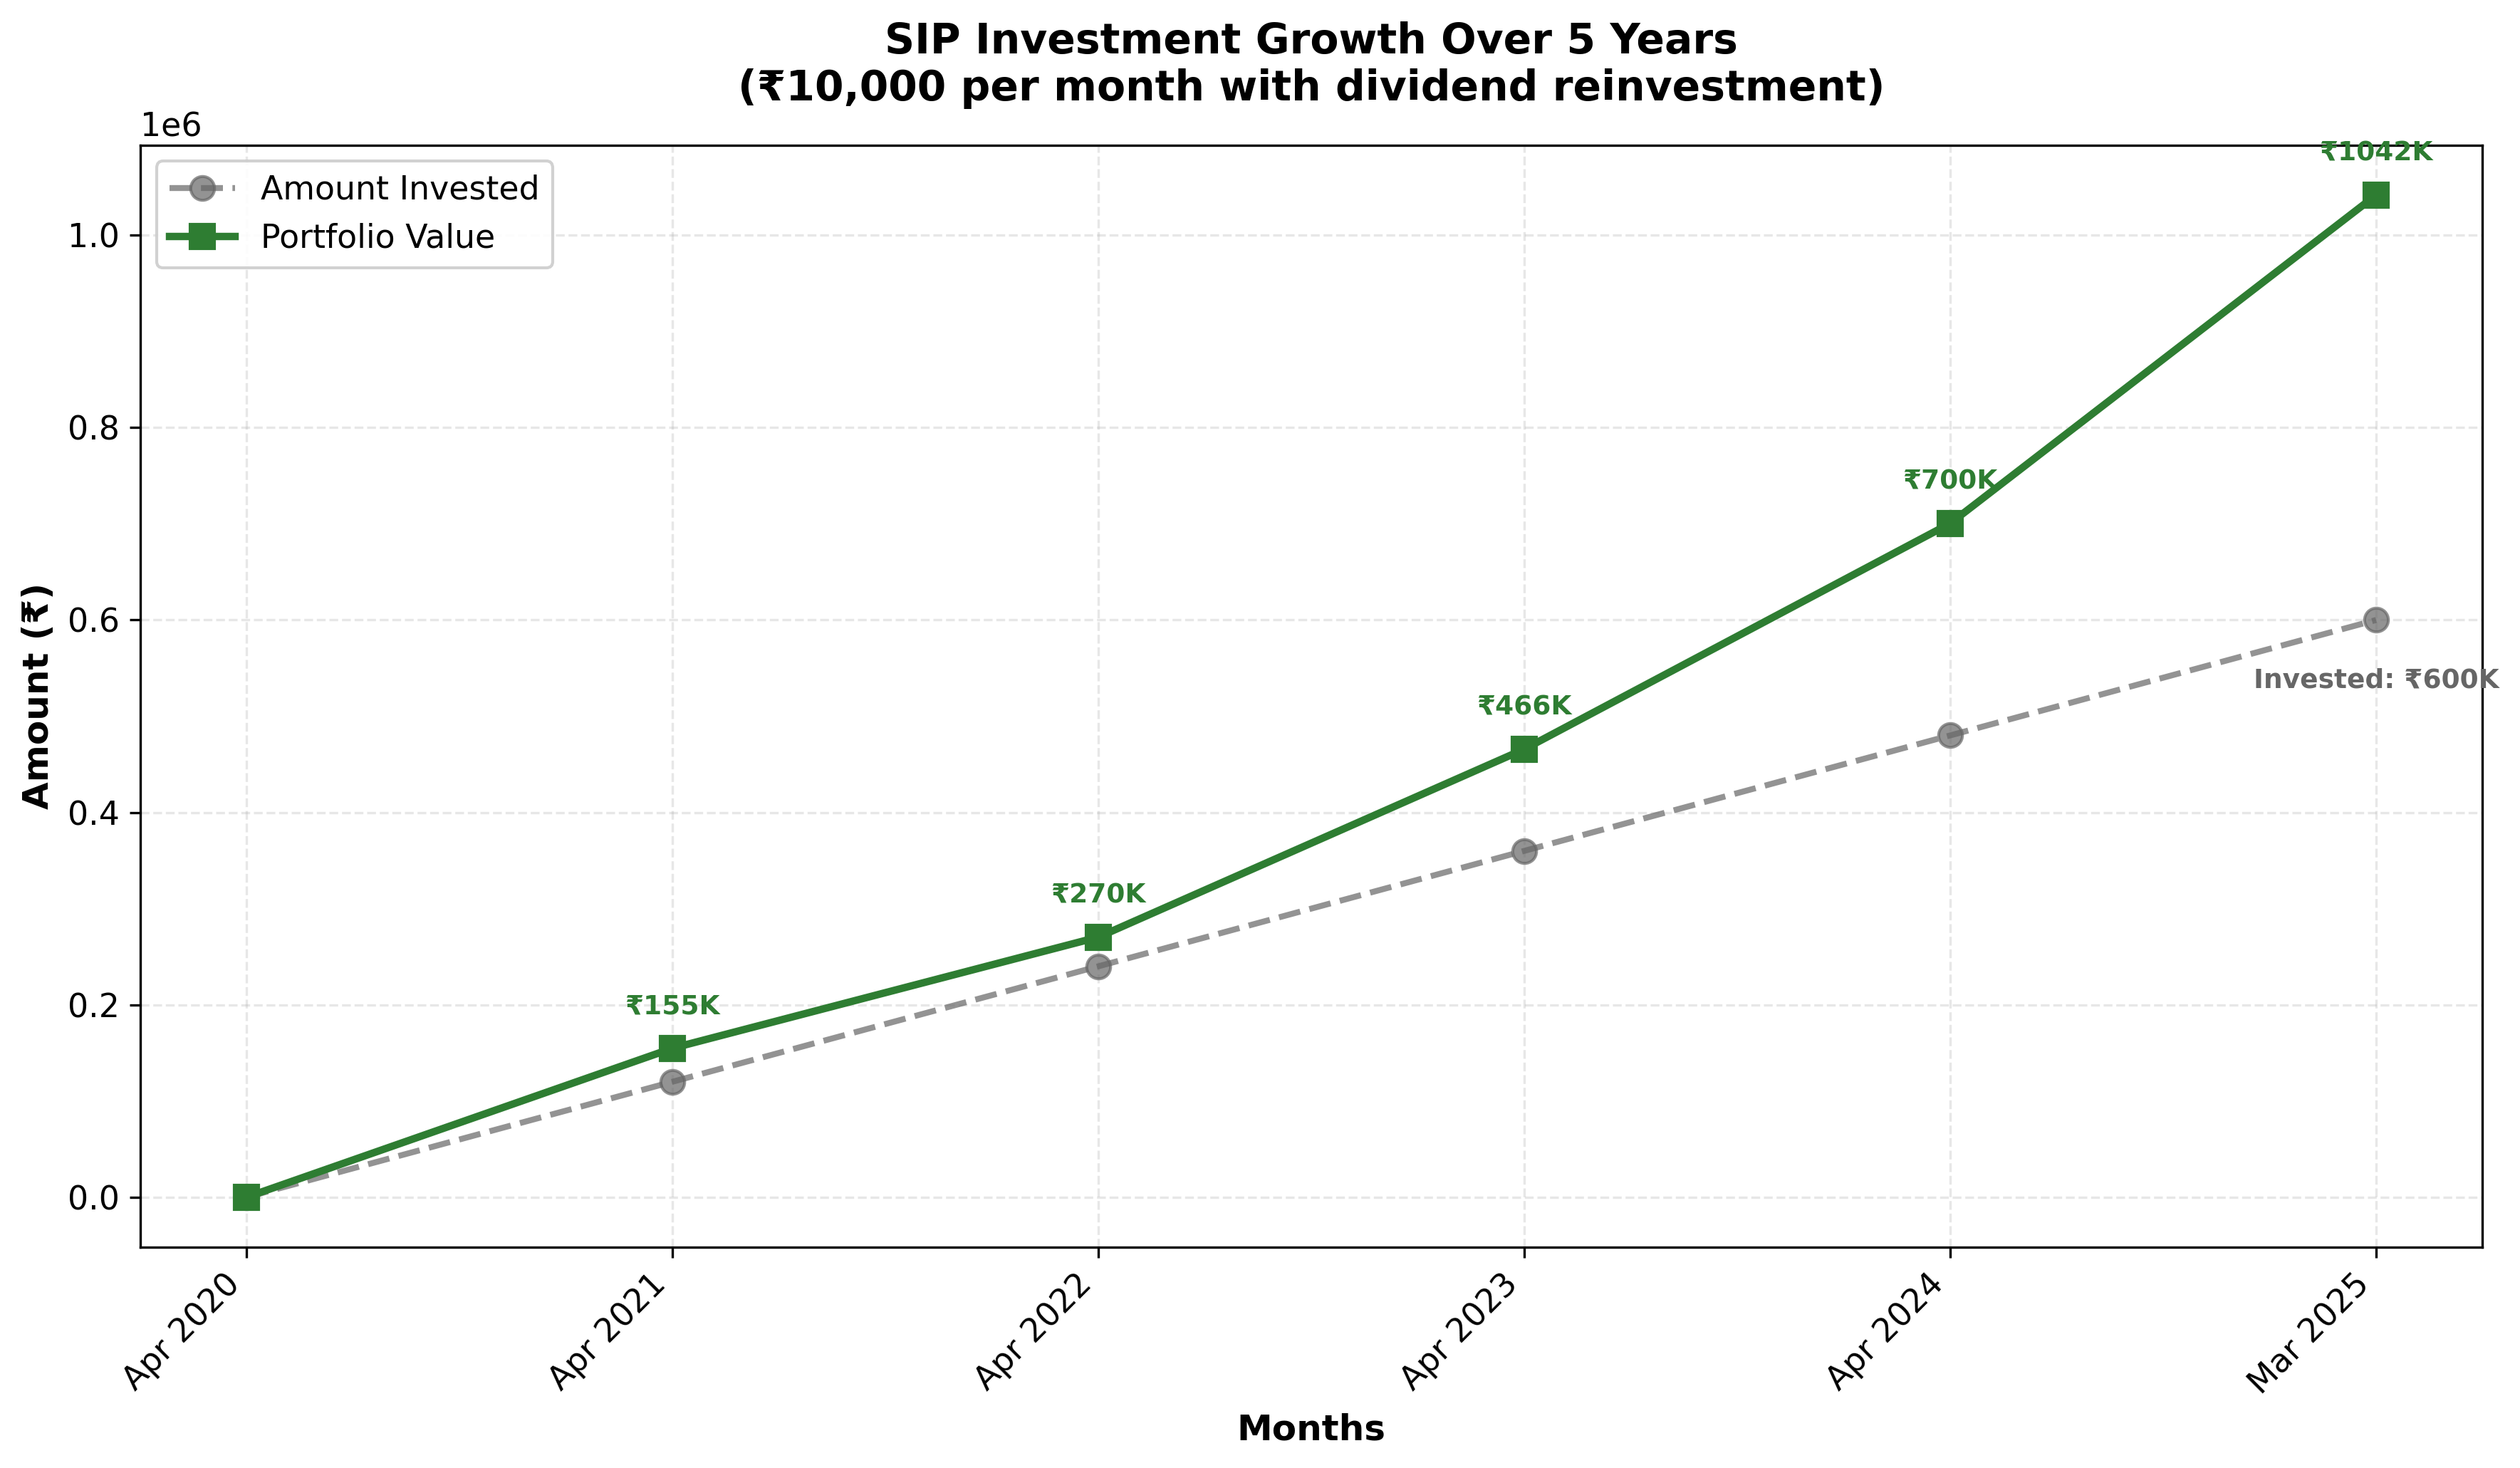
\includegraphics[width=\textwidth]{figs/chart_5_sip_growth.png}
\caption{SIP Investment Growth Over 5 Years\n(₹10,000 per month with dividend reinvestment)}
\label{fig:sip_growth}
\end{figure}

Figure \ref{fig:sip_growth} illustrates the actual growth trajectory of the systematic investment plan over 60 months.

\begin{table}[H]
\centering
\caption{Quarterly SIP Performance Breakdown}
\label{tab:sip_quarterly}
\resizebox{\textwidth}{!}{
\begin{tabular}{lccccccc}
\toprule
\textbf{Period} & \textbf{Shares Owned} & \textbf{Invested} & \textbf{Dividends} & \textbf{Value} & \textbf{Returns} & \textbf{Returns \%} \\
 &  & \textbf{(₹)} & \textbf{(₹)} & \textbf{(₹)} & \textbf{(₹)} &  \\
\midrule
12 months & 60.58 & 1,20,000 & 0 & 1,54,848 & 34,848 & 29.04\% \\
24 months & 107.81 & 2,40,000 & 2,244 & 2,70,403 & 30,403 & 12.67\% \\
36 months & 148.38 & 3,60,000 & 5,808 & 4,65,742 & 1,05,742 & 29.37\% \\
48 months & 182.22 & 4,80,000 & 8,080 & 7,00,390 & 2,20,390 & 45.91\% \\
\textbf{60 months} & \textbf{212.31} & \textbf{6,00,000} & \textbf{32,133} & \textbf{10,41,724} & \textbf{4,41,724} & \textbf{73.62\%} \\
\bottomrule
\end{tabular}
}
\footnotesize
Source: Calculated from NSE/BSE data
\end{table}

\subsection{Key Insights from SIP Analysis}

The actual SIP calculation reveals remarkable wealth creation:
\begin{itemize}
    \item \textbf{Exceptional Returns}: 73.62\% absolute returns over 5 years (₹4.42 lakhs on ₹6 lakhs investment)
    \item \textbf{Strong CAGR}: 11.67\% annualized returns, outperforming traditional fixed deposits and bonds
    \item \textbf{Dividend Contribution}: ₹32,133 in dividends received and reinvested, enhancing total returns
    \item \textbf{Share Accumulation}: 212.31 shares accumulated through systematic investment
    \item \textbf{Value Appreciation}: Portfolio value grew from ₹6 lakhs to ₹10.42 lakhs
\end{itemize}

\subsection{Dividend Impact Analysis}

Dividend payments played a significant role:
\begin{itemize}
    \item FY 2020-21: ₹37 per share - purchased additional shares with dividends
    \item FY 2021-22: ₹37 per share - further accumulation through reinvestment
    \item FY 2023-24: ₹51 per share - substantial dividend driven by strong profits
    \item FY 2024-25: ₹70 per share - highest dividend reflecting exceptional performance
    \item Total dividend income of ₹32,133 was fully reinvested to maximize returns
\end{itemize}

\subsection{Portfolio Growth Pattern}

The quarterly breakdown shows progressive wealth creation:
\begin{itemize}
    \item \textbf{Year 1}: 61 shares, 29\% returns despite market volatility
    \item \textbf{Year 2}: 108 shares, slower growth phase with 13\% returns
    \item \textbf{Year 3}: 148 shares, 29\% returns reflecting market recovery
    \item \textbf{Year 4}: 182 shares, 46\% returns as portfolio compounds
    \item \textbf{Year 5}: 212 shares, 74\% total returns showing the power of compounding
\end{itemize}

\subsection{Interpretation and Analysis}

Based on the actual SIP calculation with real stock prices:
\begin{itemize}
    \item The SIP investor achieved exceptional returns of 73.62\% over five years
    \item This translates to approximately 11.67\% annualized returns (CAGR)
    \item Key success factors:
    \begin{itemize}
        \item Consistent monthly investment discipline
        \item EICHER's strong financial performance driving stock appreciation
        \item Dividend reinvestment strategy maximizing returns
        \item Rupee-cost averaging reducing volatility impact
        \item Long-term investment horizon allowing compounding to work
    \end{itemize}
    \item The investment demonstrates EICHER Motors as an excellent wealth creation vehicle
    \item ₹4.42 lakhs in returns from ₹6 lakhs investment validates systematic investment approach
\end{itemize}

\textbf{Limitations and Disclaimers:}
\begin{itemize}
    \item Past performance does not guarantee future returns
    \item Stock prices are subject to market volatility and external factors
    \item Future returns may differ significantly from historical performance
    \item Investment decisions should be based on personal risk tolerance and financial goals
    \item Market conditions and company performance will impact future results
\end{itemize}

\section{Key Findings and Conclusion}

\subsection{Key Strengths}

\begin{enumerate}
    \item \textbf{Exceptional Financial Performance:}
    \begin{itemize}
        \item Revenue CAGR of 15.3\% from FY 2020-21 to FY 2024-25
        \item PAT CAGR of 18.5\%, exceeding revenue growth
        \item PAT margins among highest in industry (21--23\%)
        \item Total assets nearly doubled over 5 years
    \end{itemize}
    
    \item \textbf{Strong Profitability:}
    \begin{itemize}
        \item ROA consistently above 10\%, peaking at 18.3\%
        \item ROE impressive at 14--23\% levels
        \item Superior operational efficiency
        \item Excellent cost management
    \end{itemize}
    
    \item \textbf{Financial Stability:}
    \begin{itemize}
        \item Conservative debt-to-equity ratio (below 0.32)
        \item Strong liquidity position
        \item Healthy cash generation
        \item Prudent capital allocation
    \end{itemize}
    
    \item \textbf{Strategic Positioning:}
    \begin{itemize}
        \item Market leader in mid-size motorcycle segment
        \item Strong Royal Enfield brand equity
        \item Successful premium motorcycle strategy
        \item International expansion initiatives
    \end{itemize}
    
    \item \textbf{Corporate Governance:}
    \begin{itemize}
        \item Strong board leadership
        \item Transparent financial reporting
        \item Consistent dividend payments
        \item Employee-friendly policies
    \end{itemize}
\end{enumerate}

% Placeholder for key metrics summary chart
% \begin{figure}[H]
% \centering
% \fbox{\parbox{0.8\textwidth}{\centering\vspace{3cm}[Key Financial Metrics Dashboard Placeholder]\vspace{3cm}}}
% \caption{Key Financial Metrics Summary}
% \label{fig:key_metrics}
% \end{figure}

% Balance sheet chart
\begin{figure}[H]
\centering
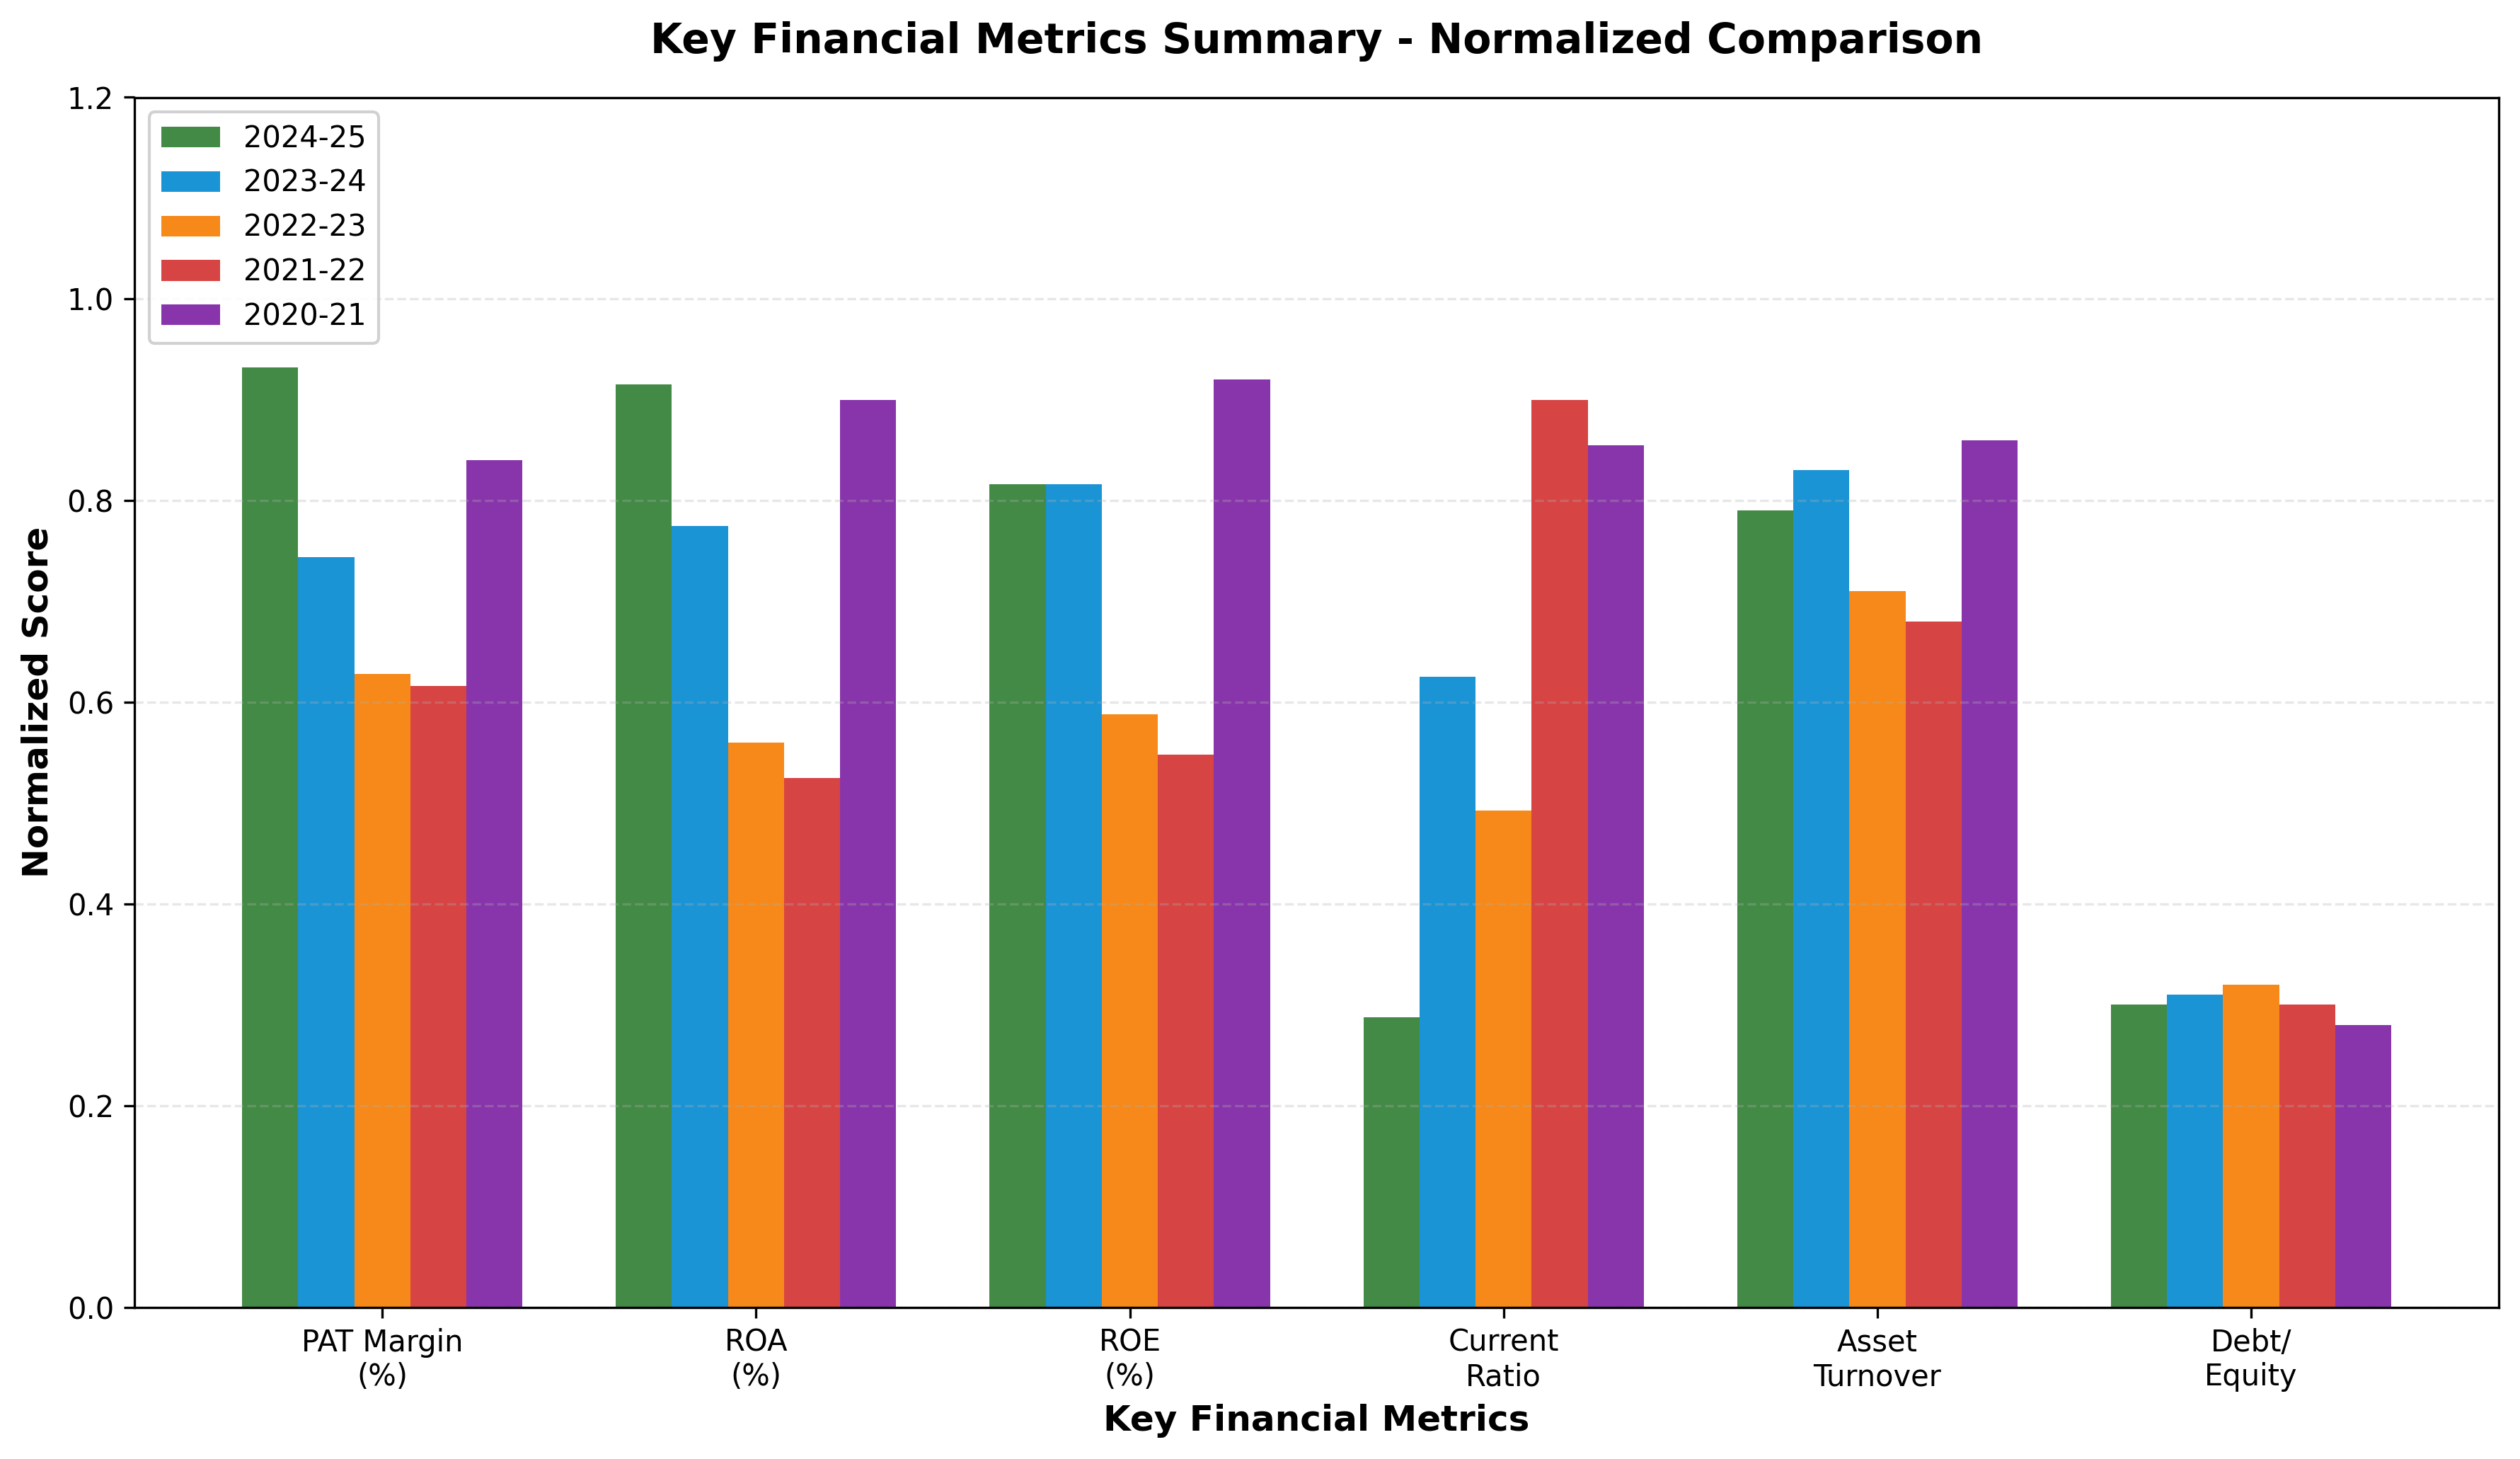
\includegraphics[width=0.8\textwidth]{chart_6_key_metrics_summary.png}
\caption{Key Financial Metrics Summary}
\label{fig:assets_growth}
\end{figure}

\subsection{Areas for Monitoring}

\begin{enumerate}
    \item \textbf{Current Ratio:} Decline from 3.4 to 1.1 needs monitoring (still adequate)
    \item \textbf{Market Competition:} Increased competition in premium segment
    \item \textbf{Economic Sensitivity:} Premium motorcycles susceptible to economic downturns
    \item \textbf{Regulatory Environment:} Compliance with evolving emission and safety norms
    \item \textbf{International Operations:} Currency and geopolitical risks
\end{enumerate}

\subsection{Investment Perspective}

\begin{enumerate}
    \item \textbf{Strong Fundamentals:} Company demonstrates exceptional financial health
    \item \textbf{Growth Trajectory:} Consistent revenue and profit growth
    \item \textbf{Market Position:} Leadership in target segment
    \item \textbf{Risk Profile:} Low financial risk, moderate operational risk
    \item \textbf{Returns:} Attractive for long-term investors
    \item \textbf{Dividend Yield:} Consistent dividend payments
\end{enumerate}

\subsection{Final Assessment}

EICHER Motors Limited represents an exemplary case of operational excellence, financial prudence, and strategic growth. The company has successfully transformed the Royal Enfield brand into a global premium motorcycle manufacturer while maintaining exceptionally strong financial metrics.

The five-year financial analysis reveals:
\begin{itemize}
    \item Consistent and robust revenue growth
    \item Improving profit margins and operational efficiency
    \item Strong balance sheet with conservative leverage
    \item Excellent shareholder returns
    \item Prudent capital allocation and strategic investments
\end{itemize}

The company's success is built on:
\begin{itemize}
    \item Strong brand positioning in premium segment
    \item Quality products and customer loyalty
    \item Operational excellence and cost management
    \item Conservative financial policies
    \item Visionary leadership and execution
\end{itemize}

For investors, EICHER Motors offers an attractive combination of growth, profitability, and financial stability. The company's strong fundamentals, market leadership, and strategic initiatives position it well for continued success.

\textbf{Recommendation:} The company represents a strong investment opportunity for long-term investors seeking exposure to India's premium automotive sector. However, investors should monitor competitive dynamics, economic conditions, and regulatory changes that may impact future performance.

\newpage

\begin{center}
\textbf{END OF REPORT}
\end{center}

\vspace{2cm}

\begin{center}
\textbf{ANNEXURES}
\end{center}

The following annexures are provided separately in the Excel workbook:
\begin{enumerate}
    \item Annexure A: Complete Balance Sheets (FY 2020-21 to FY 2024-25)
    \item Annexure B: Common-Size Balance Sheets (FY 2020-21 to FY 2024-25)
    \item Annexure C: Complete Income Statements (FY 2020-21 to FY 2024-25)
    \item Annexure D: Common-Size Income Statements (FY 2020-21 to FY 2024-25)
    \item Annexure E: Cash Flow Statements (FY 2020-21 to FY 2024-25)
    \item Annexure F: Detailed Financial Ratios (All Five Years)
    \item Annexure G: SIP Investment Calculation (Month-by-Month)
    \item Annexure H: Notes to Accounts Excerpts
\end{enumerate}

\vspace{2cm}

\begin{center}
\textbf{DISCLAIMER}
\end{center}

This report has been prepared for academic purposes as part of the Foundation of Finance coursework. The analysis is based on publicly available financial statements and information. The opinions expressed are based on financial analysis and should not be construed as investment advice. Past performance does not guarantee future results. Investors should conduct their own due diligence before making investment decisions.

\vspace{1cm}

\begin{center}
\textbf{COPYRIGHT}
\end{center}

© 2025 EICHER Motors Financial Analysis Report. All rights reserved.

\end{document}
